% SIAM Journal on Scientific Computing manuscript package.
% Compile this file from the sisc_cga directory.
\documentclass[review,hidelinks,onefignum,onetabnum,nohypdvips]{siamart251216}

% Packages used by the manuscript in addition to the SIAM class.
\usepackage{amsfonts,amssymb}
\usepackage{mathtools}
\usepackage{bm}
\usepackage{booktabs,longtable,array,multirow,tabularx}
% Preserve the SIAM class formatting for main figure and table captions.
\usepackage[caption=false,font=footnotesize]{subfig}
\usepackage[section]{placeins}
\usepackage{enumitem}
\usepackage{xcolor}
\usepackage{mdframed}
\usepackage{microtype}
\usepackage[numbers]{natbib}

\hypersetup{
  pdftitle={Chebyshev Greedy Algorithm for Nonlinear PDEs},
  pdfauthor={Ye Lin, Jiabin Yu, Youngju Lee, Jiwei Jia},
  pdfkeywords={Chebyshev greedy algorithm, nonlinear elliptic equation, p-Laplacian, natural distance}
}

\graphicspath{{figures/}{figures/cga/}{figures/baselines/}{figures/baselines_controlled/}{figures/diagnostics/}{figures/supplementary/}}

\setlist[itemize]{leftmargin=1.7em,itemsep=0.2em,topsep=0.35em}
\setlist[enumerate]{leftmargin=1.9em,itemsep=0.2em,topsep=0.35em}
\setlength{\tabcolsep}{5pt}
\emergencystretch=2em

% SIAM theorem environments already provide theorem, lemma, proposition,
% corollary, and definition. Add the manuscript-specific environments.
\newsiamthm{assumption}{Assumption}
\newsiamremark{remark}{Remark}
\crefname{assumption}{Assumption}{Assumptions}
\Crefname{assumption}{Assumption}{Assumptions}
\crefname{algorithm}{algorithm}{algorithms}
\Crefname{algorithm}{Algorithm}{Algorithms}

\newcommand{\R}{\mathbb{R}}
\newcommand{\D}{\mathcal{D}}
\newcommand{\Ppool}{\mathcal{P}}
\newcommand{\Aaudit}{\mathcal{A}}
\newcommand{\E}{\mathcal{E}}
\newcommand{\ip}[2]{\left\langle #1,#2\right\rangle}
\newcommand{\norm}[1]{\left\lVert #1\right\rVert}
\newcommand{\abs}[1]{\left\lvert #1\right\rvert}
\newcommand{\dd}{\,\mathrm{d}}
\newcommand{\spn}{\operatorname{span}}
\newcommand{\argmin}{\operatorname*{arg\,min}}
\newcommand{\eps}{\varepsilon}
\newcommand{\relu}{\operatorname{ReLU}}

% Yellow marks identify the 2026-10-01 consistency revision.  Define
% \CGAHideRevisionMarks suppresses textual marks; revised figure backgrounds
% are controlled by the artifact generator.
\ifdefined\CGAHideRevisionMarks
  \newenvironment{revision}{}{}
\else
  \newmdenv[backgroundcolor=yellow!25,linecolor=yellow!25,linewidth=0pt,
    innertopmargin=0pt,innerbottommargin=0pt,innerleftmargin=0pt,
    innerrightmargin=0pt,skipabove=0pt,skipbelow=0pt]{revision}
\fi
\makeatletter
\newcommand{\revtext}[1]{\ifdefined\CGAHideRevisionMarks #1\else
  \begingroup\dimen@=\linewidth
  \ifx\@captype\@figtxt\advance\dimen@ by -48pt\fi
  \advance\dimen@ by -2\fboxsep
  \colorbox{yellow!25}{\parbox[t]{\dimen@}{#1}}\endgroup\fi}
\makeatother

\headers{Chebyshev Greedy Algorithm for Nonlinear PDEs}{Y. Lin, J. Yu, Y. Lee, and J. Jia}

\title{Chebyshev Greedy Algorithm for Nonlinear PDEs}

\author{Ye Lin\thanks{\raggedright School of Mathematics, Jilin University, Changchun, Jilin 130012, China (\email{linye21@mails.jlu.edu.cn}, \email{yujb25@mails.jlu.edu.cn}).}
\and Jiabin Yu\footnotemark[1]
\and Youngju Lee\thanks{\raggedright Department of Mathematics, Texas State University, 601 University Drive, San Marcos, Texas 78666, United States (\email{yjlee@txstate.edu}).}
\and Jiwei Jia\thanks{\raggedright Corresponding author. School of Mathematics, Jilin University, Changchun, Jilin 130012, China, and AI for Science and Engineering Center, Shenzhen Loop Area Institute, Shenzhen, Guangdong 518048, China (\email{jiajiwei@jlu.edu.cn}).}}

\begin{document}

\maketitle

\begin{abstract}
We study the Chebyshev greedy algorithm (CGA) for convex nonlinear partial differential
equation energies by shallow \(\relu^k\) ridge functions, selected from finite candidate
pools with inexact coefficient solves. A one-step estimate separates four contributions:
coverage of the continuous dictionary by the pool, evaluation of the selection score,
radial stationarity in the active space, and the accuracy of the coefficient optimization.
For the nested spaces generated by the algorithm, an approximate-source projection bound
keeps both the source remainder and the observed orthogonal increments. For the
one-dimensional \(p=4\) energies, an exact expansion connects this bound to nonlinear
energy errors. A separate power-type decrease hypothesis gives an explicit projection
bound on a finite index range. For standard \(p\)-Laplacian energies with \(p\geq2\), an energy
exponent \(\alpha\) yields natural-distance and Sobolev exponents \(\alpha/2\) and
\(\alpha/p\).
\begin{revision}
Eight one- and two-dimensional problems illustrate the estimates.
Five of them compare finite-pool CGA prefixes with finite elements and random
features at equal retained coefficient counts. The revised comparison batch
archives every coefficient state and uses metric-specific quadrature checks.
For the two quartic auxiliary models, conservative calibration-range bounds
cover the computed errors on \(N=8\)--32. Continuing the same prefixes to
\(N=64\) with fixed constants, the normalized-innovation sufficient condition
holds on 27 and 28 of 32 transitions, respectively. These numerical checks do
not establish the same theorem guarantee throughout the continuation range
or an unconditional asymptotic convergence rate.
\end{revision}
\end{abstract}


\begin{keywords}
Chebyshev greedy algorithm; nonlinear partial differential equation; shallow neural network;
$p$-Laplacian; natural distance; finite dictionary; orthogonal greedy approximation
\end{keywords}

\begin{MSCcodes}
65N35, 65N12, 65N15, 68T07
\end{MSCcodes}

\section{Introduction}
\label{sec:introduction}

Variational formulations turn a broad class of elliptic boundary-value problems into convex energy
minimization. Classical finite elements approximate the admissible space by locally supported
polynomials, and the relation between polynomial degree, mesh scale, and degrees of freedom is well
understood \citep{BrennerScott2008}. Neural and ridge-function methods instead construct global
nonlinear trial spaces, so that the approximation problem concerns the selection and
reoptimization of atoms rather than the design of a mesh. The deep Ritz method illustrates the
reach of variational neural solvers \citep{EYu2018}. The present work analyzes a deterministic
greedy selection rule for such nonlinear elliptic energies.

Orthogonal greedy approximation (OGA) has a sharp Hilbert-space theory. Under suitable source and
entropy conditions it produces optimal approximation rates
\citep{SiegelXuOGA2022,LiSiegelEntropy2024}. Chebyshev-type greedy methods extend the basic descent
argument to convex energies in Banach spaces \citep{TemlyakovCGA2013,TemlyakovGreedy2014}, and
biorthogonal or inexact variants show how selection and correction errors enter the energy recursion
\citep{DereventsovTemlyakov2022}. These results supply the approximation theory on which the analysis
below relies. Applying them to a nonlinear partial differential equation (PDE) whose atoms are drawn
from a finite candidate pool also requires accounting for numerical quadrature, finite dictionary
approximation, and inexact coefficient minimization. The three effects are distinct: quadrature
perturbs the evaluated score, a finite pool replaces the continuous supremum by a maximum over the
pool, and an active-space solver returns only an approximate minimizer.

The dictionary used below consists of shallow \(\relu^k\) ridge functions. Here
\(\relu^k(s)=[s]_+^k\), with \([s]_+=\max\{s,0\}\), and the domain is a bounded subset of
\(\R^d\). Greedy neural training has been used successfully for PDEs
\citep{SiegelHongJinHaoXu2023}. A pool that is drawn once and then held fixed during the greedy
solve provides a way to formulate weak selection, by which we mean selection of an atom whose score is a
prescribed fraction of the best score available in the full dictionary:
\cite[Theorem~3.1]{XuXu2025} prove a convex-energy bound under Hilbert smoothness and
source/entropy assumptions, while their Theorems~5.1 and 5.2 quantify dictionary sizes that
realize weak selection. Their analysis assumes exact coefficient minimization over the active
span. The finite-pool inequality below separates the correction error from the score and coverage
errors. The universality of such constructions for nonlinear convex variational problems is
examined by \cite{BernaFalco2025}. Variation spaces and sharp entropy estimates for shallow
networks provide the source and width information used in the conditional estimates
\citep{SiegelXuVariation2023,SiegelXuSharp2024,MaoSiegelXu2026}.

The analysis has three parts. First, a one-step descent estimate separates pool
coverage, score quadrature, radial stationarity, and coefficient-correction errors.
Second, projection bounds for the computed nested spaces retain the source remainder
and the observed orthogonal increments; an exact quartic expansion connects these
bounds to nonlinear energy errors. Third, Section~\ref{sec:c5-hessian} gives a local
Hessian comparison for a concrete semilinear family and identifies the relative-score,
invariant-neighbourhood, and entropy assumptions needed for a conditional convergence
rate. The entropy estimate concerns the same projected, unrenormalized restarted
dictionary throughout. The numerical results evaluate the finite-trajectory bounds
and selected transfer quantities; they do not establish an unconditional asymptotic rate.

The convex Chebyshev algorithms of \cite{TemlyakovCGA2013,TemlyakovGreedy2014} and the inexact
weak-greedy framework of \cite{DereventsovTemlyakov2022} are closest to the present setting. The
former supplies the generic descent argument, and the latter shows how approximate selection and
correction enter an energy recurrence. The Hilbert OGA results of
\cite{SiegelXuOGA2022,LiSiegelEntropy2024} apply after a local transfer to a fixed Hessian metric;
they do not by themselves control a nonlinear PDE score or selection from a finite pool.
\cite{XuXu2025} quantify deterministic and randomized finite dictionaries under weak selection, but
they use exact active-space minimization and do not analyze a degenerate \(p\)-energy. The present
work examines the additional conditions needed for nonlinear scores, finite pools, and inexact
active-space minimization.

For \(p\)-growth energies the metric that matches the energy is not the ambient Sobolev norm. The
nonlinear map
\[
  V(\xi)=|\xi|^{(p-2)/2}\xi
\]
defines the natural distance, as in the finite-element analysis of the \(p\)-Laplacian
\citep{BarrettLiu1993,DieningKreuzer2008,LeePark2025}. A squared \(V\)-distance has the scale of an
energy gap, so an energy bound of order \(m^{-\alpha}\) gives a \(V\)-distance bound of order
\(m^{-\alpha/2}\) and, for \(p\geq2\), a \(W^{1,p}\)-error bound of order \(m^{-\alpha/p}\). This
conversion has the same form for every \(p\), although the energy exponent may depend on \(p\). We
prove the equivalence for the standard pure, regularized, and reaction \(p\)-energies and apply the
corresponding conversion to each of them.

The atomic source condition of \Cref{ass:atomic} and the directional smoothness estimate of
\Cref{ass:directional} apply to convex energies and yield an \(O(m^{-1})\) energy bound for the ideal
continuous CGA. The same arguments produce an explicit one-step inequality for finite-pool CGA, in
which four contributions appear separately: continuous-dictionary coverage, score quadrature, radial
active-space stationarity, and coefficient optimization.

Two conditional refinements use additional residual or Hessian information. The residual-comparison
estimate combines power-type convexity with a lower bound for the dictionary dual seminorm in terms
of the full dual norm. A local Hessian transfer uses coercivity, a dictionary norm comparison, and a
relative score condition to obtain a weak-OGA estimate in a frozen Hilbert metric. Neither set of
assumptions implies the other, and both are stated as conditional estimates.

The finite trajectory produced by the algorithm can also be analyzed without requiring uniform
Hessian coercivity. For a fixed finite symmetric dictionary and a fixed starting index \(m_0\), an
explicit approximation of the source with coefficient budget \(B\) and remainder \(\sigma\) gives a
projection estimate
\[
 r_{m_0+j}^2\le \sigma^2+\frac{4B^2}{\mathcal W_j},
 \qquad
 \mathcal W_j=\sum_{m=m_0}^{m_0+j-1}\frac{\underline\theta_m^2}{\ell_m^2}.
\]
Here \(r_m\) is the norm of the projection error at state \(m\), \(\ell_m\) is the innovation norm of
the selected candidate, and \(0\leq\underline\theta_m\leq\theta_m\) records the selected direction
against the best score available in the frozen dictionary. For the one-dimensional \(p=4\) energies,
whose density is quartic in the gradient, an exact expansion connects this projection error to the
energy gap. The estimate applies to the active spaces actually generated and carries a source
remainder; it does not assume that the target lies in the finite dictionary. The stronger
initial-value form of the bound is stated and evaluated numerically. A second estimate uses the
normalized innovation \(\gamma_m=\theta_m S_m/\ell_m\). If
\(\gamma_m^2\geq c_0r_m^{2+2/\alpha}\), inversion of the exact projection recurrence bounds
\(r_{m_0+j}^2\) by
\(\big(r_{m_0}^{-2/\alpha}+c_0j/\alpha\big)^{-\alpha}\). The same quartic comparison
then gives the corresponding energy and metric bounds. Each condition is evaluated from the retained
projection drops; on a finite index range, positivity alone does not single out a unique exponent.

The numerical study evaluates the estimates together with the conditions on which they rest. Eight
representative cases cover linear reaction--diffusion, cubic and hyperbolic-sine semilinear
energies, and pure, regularized, and reaction \(p\)-energies. Five of them compare finite-pool CGA, a
random-feature model (RFM), and finite elements (FEM) at equal numbers of independent coefficients.
Random features are used in their fixed-feature sense \citep{RahimiRecht2007}; conditioning of
linearized neural trial spaces is discussed by \cite{ChenChiEYang2022} and
\cite{MaoXuXu2026}. The comparison concerns coefficient counts and uses a common evaluator. It does
not attribute an unproved convergence theorem to the compared methods and does not compare
wall-clock efficiency. P1 and P3 elements provide low- and high-order mesh-based references, and P2
results are retained in the supplementary material.

For the finite-trajectory estimates we use the one-dimensional pure and regularized $p=4$
trajectories. The calibration range is $N=8$--$32$, and the subsequent range uses the same stored
prefixes from $N=33$ to $64$ with the calibration constants fixed in advance. The reported
fractions record the number of steps satisfying the stated sufficient condition on each finite
range. They provide numerical evidence on the displayed trajectory; they do not verify continuous-
dictionary coverage or an entropy estimate uniformly over increasing ranges. The approximate
source is constructed once at the starting index from the fixed candidate and auxiliary reference
dictionary. The source remainder is small relative to the starting residual but is not negligible
at the terminal scale; it therefore limits the resolution of the source upper bound without giving
a lower bound on the actual algorithmic error. Neither calculation verifies the continuous-
dictionary coverage and entropy assumptions of the Hessian-transfer result, so the measured orders
and fitted innovation powers are reported as finite-range observations.

The remainder is organized as follows. \Cref{sec:setting} defines the variational setting,
dictionaries, and algorithms. \Cref{sec:c5-descent} proves the basic descent estimates, and
\Cref{sec:pgeometry} develops the energy families and natural-distance conversion for \(p\geq2\).
\Cref{sec:c5} combines residual comparison, Hessian transfer, finite-trajectory
bounds, and fractional innovation. \Cref{sec:numerics} tests these estimates on the computed
trajectories; \Cref{sec:results} presents equal-DOF comparisons, and \Cref{sec:discussion}
summarizes the conclusions and their scope.

\section{Variational setting, dictionaries, and algorithms}
\label{sec:setting}

Let \(X\) be a real reflexive Banach space. The abstract descent results apply to a proper convex
functional \(\E:X\to(-\infty,+\infty]\), with effective domain
\(\operatorname{dom}\E=\{v\in X:\E(v)<+\infty\}\).
Differentiability is assumed on an open neighborhood of the relevant iterates in the specified
energy space, on which \(\E\) is finite and continuously Fr\'echet differentiable. For an energy
with a restricted effective domain, the additional topology and the neighborhood are stated
explicitly. When an argument invokes a Hessian, its stated neighborhood is in addition contained in
the twice differentiable part of the effective domain. Suppose that \(\E\) has a unique minimizer
\(u^*\) in the admissible space. The duality pairing between \(X^*\) and \(X\) is denoted by
\(\ip{r}{v}\), and the energy defect is
\[
  \delta(u)=\E(u)-\E(u^*), \qquad \delta_m=\delta(G_m).
\]
The examples in \Cref{sec:models} satisfy this setting after the Neumann nullspace has been
removed where necessary.

\subsection{Ridge dictionaries and admissibility}

For an integer activation order \(k\geq1\), a raw ridge atom has the form
\[
  \varphi_{w,b}(x)=\relu(w\cdot x+b)^k,
  \qquad (w,b)\in\R^d\times\R.
\]
An admissible dictionary consists of nonzero ridge functions satisfying the constraints of \(X\),
after the corresponding linear projection. We use a symmetric normalized dictionary
\(\D_X\subset X\):
\[
g\in\D_X\Longrightarrow-g\in\D_X,\qquad \norm g_X=1\quad(g\in\D_X).
\]
When density is needed, we also require \(\overline{\spn\D_X}^{\,X}=X\).
We abbreviate \(\D_X\) to \(\D\) unless a different normalization is specified.

For pure-gradient Neumann energies the admissible space is
\[
  X_{p,\circ}=\left\{v\in W^{1,p}(\Omega):\int_\Omega v\dd x=0\right\}.
\]
Each ridge is projected onto $X_{p,\circ}$ before the normalized dictionary is formed.
Since an almost constant ridge may have arbitrarily small projected norm, normalization
can amplify its derivatives. Hence uniform derivative bounds for the normalized
dictionary require a positive lower bound on the projected norms. Zero projected
atoms are excluded from the analytical dictionary; the corresponding nondegeneracy
assumption is stated whenever it is needed.

\begin{definition}[Atomic hull and atomic norm]
\label{def:atomic}
For a symmetric normalized dictionary \(\D\subset X\), define
\[
 K_1(\D)=\overline{\left\{\sum_{j=1}^Jc_jg_j:
 J<\infty,\ g_j\in\D,\ \sum_{j=1}^J\abs{c_j}\leq1\right\}}^{\,X},
\]
and
\[
 \norm{v}_{\mathcal A(\D)}=
 \inf\{B>0:v/B\in K_1(\D)\}.
\]
\end{definition}

For a bounded set \(K\subset X\), its \(n\)-th dyadic entropy number is
\[
 \varepsilon_n(K;X)=\inf\left\{h>0:\exists x_1,\ldots,x_{2^{n-1}}\in X,
 K\subset\bigcup_{j=1}^{2^{n-1}}(x_j+hB_X)\right\},\qquad n\geq1,
\]
where $B_X=\{x\in X:\norm x_X\leq1\}$. Thus the covering balls may have centers in $X$.
This $2^{n-1}$-ball convention is used throughout the manuscript. We write
$A\lesssim B$ when $A\leq CB$ with a constant independent of the iteration index; a
subscript on $\lesssim$ lists the permitted parameter dependence, and $A\simeq B$ denotes the two
corresponding inequalities.

\begin{assumption}[Atomic source]
\label[assumption]{ass:atomic}
There is a finite \(B>0\), with \(B\geq\norm{u^*}_{\mathcal A(\D)}\), such that
\(u^*/B\in K_1(\D)\).
\end{assumption}

This is a property of the target relative to the \emph{theoretically normalized} dictionary. It is not
interchangeable with the coefficient \(\ell^1\)-norm produced by a discretely normalized algorithm. In one
space dimension, \Cref{prop:1dsource} gives a sufficient condition for finite atomic norm.

\begin{proposition}[A one-dimensional \(\relu^k\) source class]
\label{prop:1dsource}
Let \(I=(0,1)\), \(k\geq1\), \(1\leq p<\infty\), and \(X=W^{1,p}(I)\). Suppose that the continuous
dictionary contains the normalized nonzero truncated powers \((x-t)_+^k/\|(\cdot-t)_+^k\|_X\),
\(0\leq t<1\), together with normalized fully active ridge functions spanning \(\mathbb P_k\). If
\(v\in W^{k+1,1}(I)\), then \(v\) belongs to the atomic space and
\[
\norm v_{\mathcal A(\D)}\leq C_{k,p}\left(
 \sum_{j=0}^k\abs{v^{(j)}(0)}+\norm{v^{(k+1)}}_{L^1(I)}\right),
\]
where \(C_{k,p}\) also accounts for the fixed exponent \(p\), the interval, and the normalization
of the raw atoms. It is a continuous-dictionary source constant and is not the coefficient
\(\ell^1\)-norm returned by a discretely normalized numerical solve.
\end{proposition}

The proof is supplied in Supplement~S4, file \texttt{A\_source\_proof\_full.tex}, and uses the integral remainder formula. Multivariate source and
entropy inputs are instead supplied by shallow-network variation-space and width theorems
\citep{SiegelXuVariation2023,SiegelXuSharp2024,MaoSiegelXu2026}; their domain and norm hypotheses
must be checked separately for each application.

\begin{lemma}[Projection and renormalization]
\label{lem:projection}
Let \(P:X\to X_0\) be bounded and linear. If a subdictionary \(\D_0\subset\D\) satisfies
\[
 0<c_0\leq\norm{Pg}_{X_0}\leq C_0<\infty\qquad(g\in\D_0),
\]
and \(\widetilde\D_0=\{Pg/\norm{Pg}_{X_0}:g\in\D_0\}\), then
\[
 P K_1(\D_0)\subset C_0K_1(\widetilde\D_0).
\]
The same computation also shows that a bounded linear map increases every entropy radius by at most
\(\norm P\), while the inverse normalization loses at most the factor \(c_0^{-1}\):
\[
 K_1(\widetilde\D_0)\subset c_0^{-1}P K_1(\D_0).
\]
\end{lemma}

\begin{proof}[Proof sketch]
For each atomic combination, write $Pg=\|Pg\|_{X_0}(Pg/\|Pg\|_{X_0})$ and use the upper and lower bounds on $\|Pg\|_{X_0}$.  Mapping a cover through $P$ multiplies its radius by at most $\|P\|$, while renormalization costs at most $c_0^{-1}$.
\end{proof}

\begin{corollary}[Transfer of source and entropy inputs]
\label{cor:projected-source-entropy}
In the setting of \Cref{lem:projection}, suppose \(u^*=Pu^\dagger\),
\(u^\dagger/B\in K_1(\D_0)\), and
\[
 \varepsilon_n(K_1(\D_0);X)\leq C_{\rm ent}n^{-\beta}.
\]
Then
\[
 \frac{u^*}{BC_0}\in K_1(\widetilde\D_0),
 \qquad
 \varepsilon_n(K_1(\widetilde\D_0);X_0)
 \leq c_0^{-1}\norm P\,C_{\rm ent}n^{-\beta}.
\]
Thus a ReLU source/convex-hull entropy theorem on an extended parameter domain passes to the projected,
renormalized feasible dictionary whenever the nondegeneracy bounds in \Cref{lem:projection} hold.
\end{corollary}

\begin{proof}[Proof sketch]
Apply the two inclusions in \Cref{lem:projection} to the atomic representation of $u^\dagger$ and to an entropy cover of $K_1(\D_0)$.  The source radius gains the factor $C_0$, and the covering radius gains $c_0^{-1}\|P\|$.
\end{proof}

\subsection{Dictionary residuals}

For \(r\in X^*\), introduce the dictionary dual seminorm
\[
  \norm r_{\D^*}=\sup_{g\in\D_X}\abs{\ip r g}.
\]
This quantity measures the derivative in the available dictionary directions. It is a seminorm;
if the dictionary has dense linear span, its vanishing implies that the derivative is zero.

\subsection{Ideal and finite-pool Chebyshev greedy algorithms}

The ideal CGA combines weak selection with exact minimization over the enlarged space.

\begin{algorithm}[htbp]
\caption{Continuous weak Chebyshev greedy algorithm}
\label{alg:continuous}
Assume \(\E(0)<\infty\), choose weakness numbers \(t_m\in(0,1]\), and set
\(G_0=0\), \(\Phi_0=\{0\}\). Given
\(G_m\) and \(\Phi_m=\spn\{g_1,\ldots,g_m\}\):
\begin{enumerate}[label=\textup{(\roman*)}]
  \item if \(\norm{\E'(G_m)}_{\D^*}=0\), stop; otherwise choose \(g_{m+1}\in\D_X\) with descent sign such that
  \[
  -\ip{\E'(G_m)}{g_{m+1}}
  \geq t_m\norm{\E'(G_m)}_{\D^*};
  \]
  \item set \(\Phi_{m+1}=\spn(\Phi_m,g_{m+1})\) and compute
  \[
    G_{m+1}=\argmin_{v\in\Phi_{m+1}}\E(v).
  \]
\end{enumerate}
\end{algorithm}

For a general continuous dictionary the supremum need not be attained. Thus \(t_m<1\) is understood as
approximate-supremum selection. The endpoint \(t_m=1\) is used only when attainment has been proved,
for example on a compact nondegenerate parameter set with continuous score. The finite-pool method
stops, with a recorded reason, if the unused pool is empty, every remaining score is below the
stationarity threshold, every candidate fails the rank or acceptance test, or the attempt budget is
reached. In an unconstrained active-space solve, changing an atom's sign leaves the span unchanged;
the descent sign required by the proof is therefore not an additional algorithmic variable.

Exact reoptimization yields the variational orthogonality
\begin{equation}
 \ip{\E'(G_m)}v=0\qquad(v\in\Phi_m).
 \label{eq:orthogonality}
\end{equation}
The second algorithm describes the computed object. It uses a finite pool \(\Ppool_m\), an evaluated
score \(\widetilde s_m\), and a correction computed to a finite tolerance.

\begin{algorithm}[htbp]
\caption{Finite-pool inexact CGA}
\label{alg:finite}
Set \(\widehat G_0=0\), \(\widehat\Phi_0=\{0\}\). At step \(m\), form a finite admissible pool
\(\Ppool_m\subset\D\). Let
\[
 s_m(g)=\abs{\ip{\E'(\widehat G_m)}g},
 \qquad \widetilde s_m(g)\geq0.
\]
Choose \(t_m^{\rm pool}\in(0,1]\) and \(\widehat g_{m+1}\in\Ppool_m\) satisfying
\[
 \widetilde s_m(\widehat g_{m+1})
 \geq t_m^{\rm pool}\max_{g\in\Ppool_m}\widetilde s_m(g),
\]
give it the true descent sign, and define
\(\widehat\Phi_{m+1}=\spn(\widehat\Phi_m,\widehat g_{m+1})\). Compute a coefficient vector whose state
obeys
\[
 \E(\widehat G_{m+1})
 \leq\inf_{v\in\widehat\Phi_{m+1}}\E(v)+\varepsilon_m^{\rm opt},
 \qquad \varepsilon_m^{\rm opt}\geq0.
\]
\end{algorithm}

\subsection{Finite-pool error quantities}
\label{sec:controlled-selection}

The continuous-dictionary supremum, the exact maximum over the finite pool, and the
numerically evaluated maximum are distinct quantities. We impose the following
score-error and pool-coverage conditions on any step for which a positive coverage
bound is used; finiteness of the pool alone does not imply a uniform positive lower bound.
\begin{align}
 \sup_{g\in\Ppool_m}\abs{\widetilde s_m(g)-s_m(g)}&\leq\xi_m,
 \label{eq:score-error}\\
 \max_{g\in\Ppool_m}s_m(g)&\geq
 \tau_m\sup_{g\in\D}s_m(g),\qquad0<\tau_m\leq1.
 \label{eq:pool-coverage}
\end{align}

\begin{lemma}[True score selected from an evaluated pool]
\label{lem:true-score}
Under \cref{eq:score-error,eq:pool-coverage},
\begin{equation}
 s_m(\widehat g_{m+1})\geq
 t_m^{\rm pool}\tau_m\norm{\E'(\widehat G_m)}_{\D^*}
 -(1+t_m^{\rm pool})\xi_m.
\label{eq:true-score-lower}
\end{equation}
\end{lemma}

\begin{proof}[Proof sketch]
The score-error bound is inserted before and after the approximate maximization, and the pool-coverage inequality replaces the finite-pool maximum by the continuous dictionary supremum.
\end{proof}

If the computed correction minimizes a discrete training objective $\E_h$, a single terminal comparison
between $\E_h$ and the analysis energy $\E$ is not a uniform error bound. The appropriate deterministic statement is
the following.

Let \(G_{m+1}^{\sharp}\) denote an exact minimizer of \(\E\) over
\(\widehat\Phi_{m+1}\). For an energy level \(\Lambda_m^E\) chosen so that both
\(G_{m+1}^{\sharp}\) and the computed state \(\widehat G_{m+1}\) are included, define the relevant sublevel
set and its active-space restriction by
\begin{equation}
 \mathcal L_m=\{v\in X:\E(v)\leq\Lambda_m^E\},
 \qquad \mathcal L_m^{\rm act}=\widehat\Phi_{m+1}\cap\mathcal L_m.
 \label{eq:active-sublevel}
\end{equation}
Thus \(\mathcal L_m^{\rm act}\) is the part of the current finite-dimensional trial space on which the
training and analysis energies must be compared; in particular,
\(\inf_{v\in\mathcal L_m^{\rm act}}\E(v)=\E(G_{m+1}^{\sharp})\).

\begin{lemma}[Transfer from the discrete energy to the analysis energy]
\label{lem:energy-transfer}
Suppose on the active-space sublevel set \(\mathcal L_m^{\rm act}\) in
\cref{eq:active-sublevel} that
\[
 \sup_{v\in\mathcal L_m^{\rm act}}
 \abs{\E_h(v)-\E(v)}\leq\zeta_m^E.
\]
If the computed state satisfies
\[
 \E_h(\widehat G_{m+1})\leq
 \inf_{v\in\mathcal L_m^{\rm act}}\E_h(v)+\varepsilon_m^{\rm opt,h},
\]
then \Cref{alg:finite} holds with
\(\varepsilon_m^{\rm opt}\leq\varepsilon_m^{\rm opt,h}+2\zeta_m^E\).
\end{lemma}

\begin{proof}[Proof sketch]
Compare the computed state with the exact active minimizer in the common sublevel set.  The uniform energy discrepancy costs at most $\zeta_m^E$ at each endpoint, so the two discrepancies add to $2\zeta_m^E$.
\end{proof}

\section{Natural geometry for variational energies}
\label{sec:pgeometry}

Let \(\Omega\subset\R^d\) be bounded, connected, and Lipschitz.
We consider diffusion and reaction equations with natural Neumann boundary conditions.
The regularization parameter \(\eps\geq0\) is fixed; the regularized model uses \(\eps>0\).
The linear and semilinear equations are
\[
-\Delta u+u=f,\qquad -\Delta u+u^3=f,\qquad -\Delta u+\sinh u=f.
\]
The standard \(p\)-structure models are
\[
-\operatorname{div}A_p(\nabla u)=f,\quad
-\operatorname{div}A_{p,\eps}(\nabla u)=f,\quad
-\operatorname{div}A_p(\nabla u)+|u|^{p-2}u=f,
\]
where \(A_p(\xi)=|\xi|^{p-2}\xi\), \(A_p(0)=0\), and
\(A_{p,\eps}(\xi)=(\eps^2+|\xi|^2)^{(p-2)/2}\xi\).
The boundary flux is zero. For the pure and regularized Neumann problems, the load annihilates constants and the zero-mean representative is used.
The equations are understood weakly when the load is not a regular function.

\subsection{Variational energies and feasible spaces}
\label{sec:models}

The three \(p\)-energies are defined in \cref{eq:pure-energy,eq:reg-energy,eq:reaction-energy}. The
remaining models have the following energies, written for \(d\leq2\):
\begin{align}
 \E_{\rm lin}(u)&=\int_\Omega\left(\frac12\abs{\nabla u}^2+
 \frac12u^2\right)\dd x-\ip fu,
 \label{eq:linear-energy}\\
 \E_{\rm cub}(u)&=\int_\Omega\left(\frac12\abs{\nabla u}^2+
 \frac14u^4\right)\dd x-\ip fu,
 \label{eq:cubic-energy}\\
 \E_{\sinh}(u)&=\int_\Omega\left(\frac12\abs{\nabla u}^2+
 \cosh u-1\right)\dd x-\ip fu.
 \label{eq:sinh-energy}
\end{align}
The pairing is the energy-space duality; for a regular load it is the corresponding integral.
The additive \(-1\) in \cref{eq:sinh-energy} normalizes the
potential and does not change the Euler--Lagrange equation.

\begin{assumption}[Data and feasible spaces for the six models]
\label[assumption]{ass:model-data}
The following model-specific conditions are imposed.
\begin{enumerate}[label=\textup{(\roman*)}]
 \item For the linear and cubic models, \(f\in (H^1(\Omega))^*\). For the sinh model, the convex
 integral functional has a load \(f\in(H^1(\Omega))^*\), and the
 integral functional is allowed to take the value \(+\infty\), its effective domain is nonempty, and
 local derivative/Hessian statements are restricted to an \(L^\infty\)-bounded neighborhood.
 \item For the pure and regularized \(p\)-energies, \(f\in X_{p,\circ}^*\), or equivalently the Neumann
 load annihilates constants before restriction to \(X_{p,\circ}\).
 \item For the reaction \(p\)-energy, \(f\in(W^{1,p})^*\). In the regularized model, the parameter
 \(\eps\) in \cref{eq:reg-energy} is fixed and positive.
\end{enumerate}
\end{assumption}

\begin{proposition}[Well-posedness]
\label{prop:wellposedness}
Under \Cref{ass:model-data}, \cref{eq:linear-energy,eq:cubic-energy,eq:sinh-energy} have unique minimizers
in \(H^1(\Omega)\); \cref{eq:pure-energy,eq:reg-energy} have unique minimizers in \(X_{p,\circ}\); and
\cref{eq:reaction-energy} has a unique minimizer in \(W^{1,p}(\Omega)\).
\end{proposition}

\begin{proof}[Proof sketch]
The quadratic, strictly convex, and $p$-growth terms give coercivity on the stated feasible spaces; strict convexity gives uniqueness.  The pure Neumann nullspace is removed by the zero-mean restriction.
\end{proof}

The local Hessian structure of each model is needed for the transfer estimates of
\Cref{sec:c5-hessian}. The bilinear forms at the exact solution are
\begin{align*}
 a_{\rm lin}(v,w)&=\int_\Omega(\nabla v\cdot\nabla w+vw)\dd x,\\
 a_{\rm cub,*}(v,w)&=\int_\Omega(\nabla v\cdot\nabla w+3(u^*)^2vw)\dd x,\\
 a_{\sinh,*}(v,w)&=\int_\Omega(\nabla v\cdot\nabla w+\cosh(u^*)vw)\dd x.
\end{align*}
For a \(p\)-diffusion density, the Hessian matrix in gradient variables is
\[
 \abs\xi^{p-2}I+(p-2)\abs\xi^{p-4}\xi\otimes\xi
\]
at nonzero \(\xi\) in the pure case, with \(\abs\xi^2\) replaced by
\(\eps^2+\abs\xi^2\) in the regularized case. The local Hessian statements that follow concern
\(p\geq2\).

\begin{proposition}[Sufficient continuous local Hessian conditions]
\label{prop:model-hessian}
In dimensions \(d\leq2\), the cubic Hessian is locally Lipschitz as a bilinear form on \(H^1\), and it
is coercive at any solution \(u^*\not\equiv0\). The sinh Hessian is coercive and is locally Lipschitz on
an \(L^\infty\)-bounded neighborhood, with the state perturbation measured in \(H^1\). For fixed
\(\eps>0\), the regularized \(p\)-Hessian is uniformly elliptic, with lower bound proportional to
\(\eps^{p-2}\); its local Lipschitz continuity is valid in the bounded-gradient topology
\(W^{1,\infty}\), not in the \(H^1\) topology asserted for the cubic model.
\end{proposition}

\begin{proof}[Proof sketch]
In dimensions $d\leq2$, Sobolev embedding controls the cubic coefficient on bounded $H^1$ neighborhoods, while an $L^\infty$ bound controls the sinh coefficient.  Differentiating the regularized radial flux gives uniform ellipticity and bounded derivative on bounded-gradient sets.
\end{proof}

\begin{proposition}[Restricted stability for the regularized \(p\)-energy]
\label{prop:regularized-restricted}
Let \(Y_M\subset W^{1,\infty}(\Omega)\) be finite dimensional and let \(\norm\cdot_{0,M}\) be any norm
on \(Y_M\). For fixed \(\eps>0\), bounded subsets of \(Y_M\) have finite restricted constants
\(L_M\) on the corresponding finite-dimensional segments. If the reference norm is chosen so that the gradient seminorm is a
norm on the feasible space, then \(\mu_M>0\). The resulting constants may depend on \(M\), the inverse
inequality on \(Y_M\), and \(\eps\).
\end{proposition}

\begin{proof}[Proof sketch]
On a bounded subset of the finite-dimensional space, norm equivalence and compactness give a finite Hessian-Lipschitz constant.  The positive ellipticity of the regularized density then yields a positive restricted coercivity constant in any reference norm that is a norm on the feasible space.
\end{proof}

The frozen Hessian is constant for the linear model, locally stable for the cubic and sinh models under the stated neighborhood restrictions, uniformly elliptic for fixed $\eps>0$ on bounded-gradient sets, and potentially degenerate for the pure and reaction $p$-models.  The transfer result therefore uses either the local Hessian hypotheses or the global $p$-geometry, according to the model.


Energy coercivity and frozen-Hessian coercivity are distinct. A positive reaction term does
not imply that the frozen \(p\)-Hessian is uniformly positive at points where both the solution and its
gradient vanish, and the continuous degeneracy of the pure model does not preclude the restricted
coercivity in the corresponding finite-dimensional metric.


\subsection{Standard \texorpdfstring{\(p\)}{p}-structure and natural distance}

For standard \(p\)-structure energies, we relate the CGA energy error to the natural distance
associated with the diffusion operator. The argument uses the pointwise structure of the density in
addition to its growth. The pointwise inequalities are standard; the step taken here is to integrate
them into an energy-to-metric estimate for the three energy families below, together with the
matching \(W^{1,p}\) conversion. Let \(\Omega\subset\R^d\) be bounded, connected, and Lipschitz, and
let \(p\geq2\). On the zero-mean space \(X_{p,\circ}\), define the pure and regularized energies
\begin{align}
 \E_p(u)&=\int_\Omega\frac1p\abs{\nabla u}^p\dd x-\ip fu,
 \label{eq:pure-energy}\\
 \E_{p,\eps}(u)&=\int_\Omega
 \frac{(\eps^2+\abs{\nabla u}^2)^{p/2}-\eps^p}{p}\dd x-\ip fu,
 \qquad\eps>0.
 \label{eq:reg-energy}
\end{align}
On \(W^{1,p}(\Omega)\), define the reaction energy
\begin{equation}
 \E_{p,R}(u)=\int_\Omega\left(\frac1p\abs{\nabla u}^p+
 \frac1p\abs u^p\right)\dd x-\ip fu.
 \label{eq:reaction-energy}
\end{equation}

For a differentiable convex functional \(F\), its Bregman divergence is
\begin{equation}
 D_F(u,v)=F(u)-F(v)-\ip{F'(v)}{u-v}\geq0.
 \label{eq:bregman-definition}
\end{equation}
It measures the part of the energy increment not accounted for by the tangent functional at \(v\). In
general \(D_F(u,v)\neq D_F(v,u)\), so it is not a metric. The same notation is used pointwise for a
convex density: \(D_\phi(a,b)=\phi(a)-\phi(b)-\nabla\phi(b)\cdot(a-b)\).

For scalar arguments set \(V(s)=\abs{s}^{(p-2)/2}s\), and for vector arguments set
\[
 V(\xi)=\abs\xi^{(p-2)/2}\xi,
 \qquad
 V_\eps(\xi)=(\eps^2+\abs\xi^2)^{(p-2)/4}\xi.
\]
The corresponding natural distances are
\begin{align*}
 d_V(u,v)^2&=\norm{V(\nabla u)-V(\nabla v)}_{L^2}^2,\\
 d_{V,\eps}(u,v)^2&=\norm{V_\eps(\nabla u)-V_\eps(\nabla v)}_{L^2}^2,\\
d_{V,R}(u,v)^2&=d_V(u,v)^2+
 \norm{V(u)-V(v)}_{L^2}^2.
\end{align*}
We use \(\E_\bullet\) and \(d_{V,\bullet}\) only as paired abbreviations for one of
\((\E_p,d_V)\), \((\E_{p,\eps},d_{V,\eps})\), or \((\E_{p,R},d_{V,R})\). The scalar map applies to
the reaction term and the vector map to gradients. The map \(V\) turns the weighted quadratic
structure of a \(p\)-operator into an \(L^2\)-type distance
\citep{BarrettLiu1993,DieningKreuzer2008,LeePark2025}.

Throughout this section, \(A\lesssim_p B\) means \(A\leq C(p)B\), and \(A\simeq_p B\) means that
both inequalities hold with positive constants depending only on \(p\); a further subscript lists
any additional permitted dependence.

\begin{lemma}[Pointwise \(p\)-structure]
\label{lem:pstructure}
For \(p\geq2\), constants depending only on \(p\) satisfy, for every
\(a,b\in\R^d\),
\begin{align}
 &\frac{\abs a^p}{p}-\frac{\abs b^p}{p}
 -\abs b^{p-2}b\cdot(a-b)
 \simeq_p(\abs a+\abs b)^{p-2}\abs{a-b}^2
 \simeq_p\abs{V(a)-V(b)}^2,
 \label{eq:pstructure}\\
 &\abs{a-b}^p\lesssim_p\abs{V(a)-V(b)}^2.
 \label{eq:pcontrol}
\end{align}
The analogous statements hold for the regularized density and \(V_\eps\), with \(\eps>0\) fixed.
\end{lemma}

\begin{proof}[Proof sketch]
These are the standard monotonicity and radial-growth inequalities for $\xi\mapsto|\xi|^{p-2}\xi$; the regularized statements follow from the same calculation with $\eps^2+|\xi|^2$.
\end{proof}

\begin{theorem}[Energy--natural-distance equivalence]
\label{thm:energy-v}
For each of the three energy--space pairs
\[
 (\E_p,X_{p,\circ}),\qquad(\E_{p,\eps},X_{p,\circ}),\qquad
 (\E_{p,R},W^{1,p}(\Omega)),
\]
let \(u^*\) be the minimizer. Then, for every admissible \(u\), respectively,
\begin{align}
 \E_p(u)-\E_p(u^*)&\simeq_p d_V(u,u^*)^2,
 \label{eq:pure-equiv}\\
 \E_{p,\eps}(u)-\E_{p,\eps}(u^*)&\simeq_{p,\eps}d_{V,\eps}(u,u^*)^2,
 \label{eq:reg-equiv}\\
 \E_{p,R}(u)-\E_{p,R}(u^*)&\simeq_p d_{V,R}(u,u^*)^2.
 \label{eq:reaction-equiv}
\end{align}
In the corresponding spaces,
\begin{equation}
 \norm{u-u^*}_{W^{1,p}}^p
 \lesssim_{p,\Omega,\eps}d_{V,\bullet}(u,u^*)^2,
 \label{eq:w1p-control}
\end{equation}
where the constants in the pure and reaction cases are independent of \(\eps\).
\end{theorem}

\begin{proof}[Proof sketch]
Integrate the pointwise Bregman equivalences for the gradient and reaction terms.  The weak optimality of $u^*$ cancels the load term, and Poincare's inequality controls the zero-mean representative in the pure and regularized cases.
\end{proof}

\begin{corollary}[Metric exponents]
\label{cor:metric-rates}
Fix any one of the three energy--space--distance triples in \Cref{thm:energy-v}. If a sequence
\(G_m\) in that feasible space satisfies
 \begin{equation}
 \E_\bullet(G_m)-\E_\bullet(u^*)=O(m^{-\alpha})
 \label{eq:assumed-energy-rate}
 \end{equation}
for some \(\alpha>0\), then
 \begin{equation}
 d_{V,\bullet}(G_m,u^*)=O(m^{-\alpha/2}),
 \qquad
 \norm{G_m-u^*}_{W^{1,p}}=O(m^{-\alpha/p}).
\label{eq:metric-rates}
 \end{equation}
\end{corollary}

\begin{proof}[Proof sketch]
Apply the two-sided energy--distance equivalence and the $W^{1,p}$ control in \Cref{thm:energy-v} to the assumed energy bound, then take the corresponding square or $p$-th root.
\end{proof}

\begin{remark}[Scope]
The corollary is restricted to the three standard \(p\)-Laplacian-type energies just defined. Linear,
cubic, and hyperbolic-sine energies have their own quadratic or local-Hessian geometry and are not
instances of this statement merely because they are convex. Conversely, an unspecified energy with
\(p\)-growth need not satisfy the Bregman--\(V\) equivalence in \Cref{lem:pstructure}.
\end{remark}

\def\CGAChapterFiveEmbedded{1}% Condensed main-text theory for the SISC-length manuscript.
% The full derivations are retained in supplement/S4_theory_details.tex.
\ifdefined\CGAChapterFiveEmbedded
\else
\documentclass[11pt]{article}
\usepackage[a4paper,margin=25mm]{geometry}
\usepackage{amsmath,amssymb,amsthm,mathtools,booktabs,microtype,enumitem}
\usepackage[hidelinks]{hyperref}
\def\CGAChapterFiveStandalone{1}
\newtheorem{theorem}{Theorem}[section]
\newtheorem{lemma}[theorem]{Lemma}
\newtheorem{proposition}[theorem]{Proposition}
\newtheorem{corollary}[theorem]{Corollary}
\newtheorem{assumption}[theorem]{Assumption}
\theoremstyle{remark}\newtheorem{remark}[theorem]{Remark}
\begin{document}\setcounter{section}{4}
\fi
\providecommand{\cE}{\mathcal E}
\providecommand{\cD}{\mathcal D}
\providecommand{\cP}{\mathcal P}
\providecommand{\cK}{\mathcal K}
\providecommand{\cnorm}[1]{\left\lVert#1\right\rVert}
\providecommand{\cabs}[1]{\left|#1\right|}
\providecommand{\cinner}[2]{\left\langle#1,#2\right\rangle}
\providecommand{\cR}{\mathbb R}
\providecommand{\cdd}{\,\mathrm d}
\ifdefined\CGAChapterFiveStandalone
  \newcommand{\CGAHLDreference}{Section~3}
  \newcommand{\CGAEnergyMetricReference}{the energy--distance theorem and metric corollary in Section~4}
  \newcommand{\CGAEnergyTheoremReference}{the energy--distance theorem in Section~4}
\else
  \newcommand{\CGAHLDreference}{Section~\ref{sec:c5-descent}}
  \newcommand{\CGAEnergyMetricReference}{Theorem~\ref{thm:energy-v} and Corollary~\ref{cor:metric-rates}}
  \newcommand{\CGAEnergyTheoremReference}{Theorem~\ref{thm:energy-v}}
\fi

\section{Conditional convergence and finite-trajectory projection bounds}
\label{sec:c5}

The analysis separates finite-pool descent from approximation in a frozen
Hilbert metric.  Pool coverage, score evaluation, radial stationarity, and
coefficient correction enter the first part; nested-space projection and local
Hessian information enter the second.  The connection is conditional, and the
quartic models additionally admit an exact energy identity.

Throughout, $m$ counts accepted independent directions, $m_0$ is a starting
index, $\widehat G_m$ is a computed state, $G_m^\sharp$ an exact active-space
minimizer, and $z_m$ a frozen orthogonal projection.  All derivatives act on
the specified feasible linear space.

\subsection{Finite-pool descent and residual comparison}
\label{sec:c5-descent}
\label{sec:descent}

Let $X$ be a real Banach space, $\cE:X\to\cR$ convex and differentiable, and
$u^*$ a minimizer.  For a symmetric unit dictionary $\cD_X$, set
\[
 \widehat\delta_m=\cE(\widehat G_m)-\cE(u^*),\qquad
 S_m^X=\sup_{g\in\cD_X}|\cinner{\cE'(\widehat G_m)}g|.
\]
For a finite pool $\cP_m\subset\cD_X$ and $0<t_m^{\rm pool}\le1$, write
\[
 |\widetilde s_m(g)-s_m(g)|\le\xi_m,\qquad
 \widetilde s_m(g_{m+1})\ge t_m^{\rm pool}\max_{g\in\cP_m}\widetilde s_m(g),
\]
where $s_m(g)=|\cinner{\cE'(\widehat G_m)}g|$.  Its continuous coverage is
$\tau_m=\max_{\cP_m}s_m/S_m^X$ when $S_m^X>0$, and we set $\tau_m=1$
when $S_m^X=0$.
\begin{assumption}[Directional quadratic upper bound]
\label[assumption]{ass:directional}
For some $L>0$, every $m$, every $g\in\cD_X$, and $|\lambda|\leq1$,
\begin{equation}
 \cE(\widehat G_m+\lambda g)\leq\cE(\widehat G_m)+\lambda\cinner{\cE'(\widehat G_m)}g+\tfrac L2\lambda^2,
\label{eq:c5-directional}
\end{equation}
\end{assumption}
Assume that the expanded active space contains the signed step used below and that
the inexact active correction satisfies
\[
 \cE(\widehat G_{m+1})\leq
 \inf_{v\in\widehat\Phi_{m+1}}\cE(v)+\varepsilon_m^{\rm opt},
 \qquad \varepsilon_m^{\rm opt}\geq0.
\]
Define
$H_L(a)=\max_{0\le\lambda\le1}(\lambda a-L\lambda^2/2)$.

\begin{proposition}[Finite-pool descent]
\label{prop:c5-descent}
\label{thm:inexact}
Under these conditions,
\begin{equation}
 \widehat\delta_{m+1}\leq\widehat\delta_m-H_L(a_m)+\varepsilon_m^{\rm opt},\qquad
 a_m=\left[t_m^{\rm pool}\tau_m S_m^X-(1+t_m^{\rm pool})\xi_m\right]_+ .
 \label{eq:c5-descent}
\end{equation}
\end{proposition}
\begin{proof}
The score error is inserted before and after the finite-pool maximization.  Testing the enlarged active space with a signed step of length $\min\{1,a_m/L\}$ gives the displayed decrease, and the correction error is added once.
\end{proof}

If $B_{\rm src}>0$, $u^*/B_{\rm src}$ belongs to the closed absolutely convex hull of $\cD_X$, and the
radial defect satisfies $|\cinner{\cE'(\widehat G_m)}{\widehat G_m}|\leq\eta_m^{\rm rad}$, convexity gives
\begin{equation}
 \widehat\delta_m\leq\eta_m^{\rm rad}+B_{\rm src}S_m^X.
 \label{eq:c5-atomic}
\end{equation}
Thus radial stationarity is distinct from score error and correction error.

\begin{lemma}[Nonautonomous scalar recurrence]
\label{lem:c5-recurrence}
If $x_m\ge0$ and $x_{m+1}\le x_m-b_mx_m^q$ with $q>1$ and $b_m\ge0$, then, for
$x_0>0$,
\begin{equation}
 x_n\le\left[x_0^{1-q}+(q-1)\sum_{m=0}^{n-1}b_m\right]^{-1/(q-1)}.
 \label{eq:c5-recurrence}
\end{equation}
If $x_0=0$, the sequence vanishes.
\end{lemma}
\begin{proof}
Apply convexity to $x\mapsto x^{1-q}$ while the sequence is positive and sum the resulting increments; once a term vanishes, nonnegativity gives the remaining cases.
\end{proof}

The atomic baseline follows by assuming, for $m\ge m_0$,
\[
 t_m^{\rm pool}\tau_m\ge\underline t>0,\qquad
 \eta_m^{\rm rad}+
 \frac{B_{\rm src}(1+t_m^{\rm pool})}{t_m^{\rm pool}\tau_m}\xi_m
 \le\vartheta\widehat\delta_m,
 \qquad\varepsilon_m^{\rm opt}\le\zeta H_L(a_m),
\]
with $0\le\vartheta,\zeta<1$. Equation~\eqref{eq:c5-atomic} gives
$a_m\ge\underline t(1-\vartheta)\widehat\delta_m/B_{\rm src}$.
Descent is monotone and $H_L(a)\ge a^2/(2\max\{L,A\})$ for $0\le a\le A$;
applying this to the displayed lower bound for $a_m$ gives
$\widehat\delta_{m+1}\le\widehat\delta_m-c\widehat\delta_m^2$ with $c>0$.
Lemma~\ref{lem:c5-recurrence} yields
$\widehat\delta_m=O((m-m_0+1)^{-1})$ on the tail. The ideal continuous method
is the case $\tau_m=1$ and $\xi_m=\eta_m^{\rm rad}=\varepsilon_m^{\rm opt}=0$,
with selection weakness bounded below.

\begin{theorem}[Conditional residual-comparison rate]
\label{thm:c5-visible}
Let $p>2$, $c_U>0$, and $\kappa_0>0$. Suppose
$\widehat\delta_m\ge c_U\|\widehat G_m-u^*\|_X^p$ and
$S_m^X\ge\kappa_0(m+1)^{-\chi}\|\cE'(\widehat G_m)\|_{X^*}$ with
$0\le\chi<1/2$.  Assume, uniformly in $m$, that
\[
 t_m^{\rm pool}\tau_m\ge\underline t>0,\qquad
 (1+t_m^{\rm pool})\xi_m\leq\vartheta t_m^{\rm pool}\tau_m S_m^X,
 \quad 0\leq\vartheta<1,
\]
and that the correction error satisfies
$\varepsilon_m^{\rm opt}\leq\zeta H_L(a_m)$ with $0\leq\zeta<1$.
Together with the directional bound above, these conditions give
\begin{equation}
 \widehat\delta_m=O\big((m+1)^{-p(1-2\chi)/(p-2)}\big).
 \label{eq:c5-visible-rate}
\end{equation}
\end{theorem}
\begin{proof}
Convexity and the lower bound on $\widehat\delta_m$ give
$\|\cE'(\widehat G_m)\|_{X^*}\geq c_U^{1/p}\widehat\delta_m^{(p-1)/p}$.
The pool and error assumptions therefore give a selected score bounded below by
a fixed multiple of $(m+1)^{-\chi}\widehat\delta_m^{(p-1)/p}$.
Descent and absorption give monotonicity. The lower score bound is therefore
bounded above by a fixed $A$, so the same quadratic lower bound for $H_L$
gives Lemma~\ref{lem:c5-recurrence} with $q=2(p-1)/p$ and
$b_m\asymp(m+1)^{-2\chi}$. The sum grows as $m^{1-2\chi}$.
\end{proof}

\subsection{Energy and natural distance}
\label{sec:c5-natural}

For the standard pure, regularized, and reaction $p$-energies, \CGAEnergyMetricReference gives
energy--distance equivalence and the $W^{1,p}$ conversion.  Hence an energy estimate
$\widehat\delta_m=O(m^{-\alpha})$ implies
\[
 d_{V,\bullet}(\widehat G_m,u^*)=O(m^{-\alpha/2}),\qquad
 \|\widehat G_m-u^*\|_{W^{1,p}}=O(m^{-\alpha/p}).
\]
The statement is restricted to the three specified energy densities.

\subsection{Local Hessian transfer and the same-dictionary requirement}
\label{sec:c5-hessian}

The local transfer result is the main conditional refinement. Let $H$ be a
Hilbert space on which $\cE$ is twice Fr\'echet differentiable in an open
convex neighborhood of its minimizer $u^*$. Let $A_*=\cE''(u^*)$ be bounded,
symmetric, and coercive, and set
$a_*(v,w)=\langle A_*v,w\rangle$, $\|v\|_*^2=a_*(v,v)$.
Assume the closed ball $\|u-u^*\|_*\le R_*$ lies in this neighborhood and
\begin{equation}
 |\langle[\cE''(u)-A_*]v,w\rangle|
 \le L_*\|u-u^*\|_*\|v\|_*\|w\|_*,\qquad L_*R_*\le\tfrac12 .
 \label{eq:c5-hessian}
\end{equation}
For a finite-dimensional space $\Phi$, let $z_\Phi$ be the frozen $A_*$-projection and
$G_\Phi^\sharp$ the exact energy minimizer, both inside this ball.

\begin{lemma}[Taylor and projection estimates]
\label{lem:c5-projection}
Under \eqref{eq:c5-hessian}, for $u$ in this ball,
\begin{align}
 \left|\cE(u)-\cE(u^*)-\tfrac12\|u-u^*\|_*^2\right|&\le\tfrac{L_*}{6}\|u-u^*\|_*^3,\\
 \|\cE'(u)-A_*(u-u^*)\|_{*'}&\le\tfrac{L_*}{2}\|u-u^*\|_*^2,\\
 \|G_\Phi^\sharp-z_\Phi\|_*&\le L_*\|z_\Phi-u^*\|_*^2.
 \label{eq:c5-proj}
\end{align}
\end{lemma}
\begin{proof}
Taylor's formula gives the first two inequalities.  The third follows by testing the active-space first-order condition with $G_\Phi^\sharp-z_\Phi$ and absorbing the term $L_*R_*\|G_\Phi^\sharp-z_\Phi\|_*^2$.
\end{proof}

Assume the algorithmic dictionary $\cD_X\subset H$ satisfies
\begin{equation}
 0<c_*\le\|g\|_*\le C_*<\infty\quad(g\in\cD_X),
\qquad \cD_* = \left\{g/\|g\|_*:g\in\cD_X\right\}.
 \label{eq:c5-bridge}
\end{equation}
Let $\Phi_{m+1}=\Phi_m+\operatorname{span}\{g_{m+1}\}$, where
$g_{m+1}\in\cD_X\setminus\Phi_m$, and let $P_m$ be the $a_*$-orthogonal
projection onto $\Phi_m$. Set $z_m=P_mu^*$ and define
$S_m^*=\sup_{d\in\cD_*}|\langle A_*(z_m-u^*),d\rangle|$.  At the exact
active-space minimizer $G_m^\sharp$ define the score defect
\[
 \eta_m^H=\sup_{g\in\cD_X}
 \left|\langle\cE'(G_m^\sharp),g\rangle-a_*(z_m-u^*,g)\right|.
\]
Lemma~\ref{lem:c5-projection} yields
$\eta_m^H\le C_{T}\|z_m-u^*\|_*^2$ on the stated ball, with $C_T$ uniform
over the specified dictionary.

\begin{proposition}[Relative score transfer]
\label{prop:c5-transfer}
If nonlinear selection at $G_m^\sharp$ over $\cD_X$ has strength
$t\in(0,1]$ and $0<t_0<tc_*/C_*$, then
\begin{equation}
 (1+t)\eta_m^H\le (tc_*-t_0C_*)S_m^*
 \label{eq:c5-relative}
\end{equation}
implies that the selected direction satisfies
\[
 \left|a_*(z_m-u^*,g_{m+1}/\|g_{m+1}\|_*)\right|\ge t_0S_m^*.
\]
\end{proposition}
\begin{proof}
The selected unnormalized frozen score is bounded below by
$t c_*S_m^*-(1+t)\eta_m^H$; division by the selected frozen norm costs at most
$C_*$.  This proves the claim.
\end{proof}

For a concrete semilinear family, take $H=H^1(0,1)$ and
\[
 \cE_\lambda(u)=\int_0^1\left(\tfrac12|u'|^2+\tfrac12u^2+\tfrac\lambda4u^4\right)\cdd x-\ell(u),
 \qquad \lambda\ge0,
\]
For $k\ge2$ and $0<a<b<1$, use the dictionary
$\cD_X=\{\pm g_t:t\in[a,b]\}$, where
$g_t=(x-t)_+^k/\|(\cdot-t)_+^k\|_{H^1}$.
Choose a finite signed measure $\mu$ with total variation at most $B_{\rm src}>0$,
set $u^*=\int_a^b g_t\,\mathrm d\mu(t)$, and define the variational load by
$\ell(v)=\int_0^1(u^{*\prime}v'+u^*v+\lambda(u^*)^3v)\,\mathrm dx$.
This construction makes $u^*$ the unique minimizer; it does not impose
homogeneous Neumann data. The parameter restriction makes the dictionary compact.
Let $C_{\rm emb}$ satisfy $\|v\|_\infty\le C_{\rm emb}\|v\|_{H^1}$
and put $M_*=\|u^*\|_\infty$. Directly bounding
$3\lambda(u^2-(u^*)^2)vw$ gives
\[
 L_\lambda=3\lambda C_{\rm emb}(C_{\rm emb}R_*+2M_*),\qquad
 c_*=1,\quad C_\lambda=(1+3\lambda M_*^2)^{1/2},\quad
 B_\lambda=C_\lambda B_{\rm src}.
\]
Thus $u^*\in B_\lambda\cK_1(\cD_*)$. With
$C_{T,\lambda}=L_\lambda[1+\tfrac12(1+L_\lambda R_*)^2]$,
the projection lemma gives $\eta_m^H\le C_\lambda C_{T,\lambda}r_m^2$,
where $r_m=\|u^*-z_m\|_*$. Orthogonality and the source representation give
$S_m^*\ge r_m^2/B_\lambda$. Hence a sufficient relative-score condition is
\begin{equation}
\Delta_\lambda=(tc_*-t_0C_\lambda)
 -(1+t)C_\lambda^2C_{T,\lambda}B_{\rm src}>0,
 \label{eq:c5-small-lambda-score}
\end{equation}
with $L_\lambda R_*\le1/2$. Invariance of the ball and a quantitative
entropy bound remain additional requirements.

To make the entropy-to-rate step explicit, fix a restart index $m_0$ and set
$Q_0=I-P_{m_0}$, $H_0=Q_0H$, $f_0=Q_0u^*$, and
$\cD_{\rm rst}=Q_0\cD_*\setminus\{0\}$.  The projected atoms are not renormalized.
Suppose $K=\cK_1(\cD_{\rm rst})$ is compact and $f_0\in B_*K$, $B_*>0$.
For weak OGA of strength $t_0$ in $H_0$, let $d_i\in\cD_{\rm rst}$ be
the selected atoms and $\Pi_j$ the orthogonal projection onto their first $j$
spans, with $\Pi_0=0$. The bounded-atom entropy argument of
\cite[Theorem~4.2]{LiSiegelEntropy2024} gives
\begin{equation}
 \|f_0-\Pi_jf_0\|_*
 \leq \frac{B_*}{t_0}\frac{(j!V_j)^{1/j}}{\sqrt j}
 \varepsilon_{j+1}(K;H_0),
 \qquad V_j=\frac{\pi^{j/2}}{\Gamma(j/2+1)}.
 \label{eq:c5-entropy}
\end{equation}
Indeed, writing $y_i=\|f_0-\Pi_if_0\|_*^2$ and
$\ell_i^{\rm rst}=\|(I-\Pi_{i-1})d_i\|_*$, the source and weak selection give
\[
 y_i\le y_{i-1}-\frac{t_0^2y_{i-1}^2}{B_*^2(\ell_i^{\rm rst})^2},
 \qquad
 y_j\le\frac{B_*^2}{t_0^2j}
       \left(\prod_{i=1}^j\ell_i^{\rm rst}\right)^{2/j}.
\]
The second bound follows by reciprocation and the arithmetic--geometric mean
inequality while the errors are positive. The cross-polytope generated by
$\{\pm d_1,\ldots,\pm d_j\}$ lies in $\Pi_jK$ and has volume
$(2^j/j!)\prod_i\ell_i^{\rm rst}$.
A cover of $K$ by $2^j$ balls yields
$\prod_i\ell_i^{\rm rst}\le j!V_j\varepsilon_{j+1}(K;H_0)^j$,
by taking the infimum over covering radii. This proves \eqref{eq:c5-entropy};
zero errors persist. Stirling's formula bounds $(j!V_j)^{1/j}/\sqrt j$
uniformly.

\begin{theorem}[Conditional Hessian transfer after restart]
\label{thm:c5-hessian}
Assume \eqref{eq:c5-hessian}, \eqref{eq:c5-bridge}, and exact active-space
minimization. At each step $m_0\le m<m_0+J$, suppose nonlinear selection has
strength at least $t$ and \eqref{eq:c5-relative} holds with the same $t_0>0$.
Assume the exact minimizers and frozen projections remain in the Hessian ball
for $m_0\le m\le m_0+J$, $K$ is compact, and
\[
 f_0\in B_*\cK_1(\cD_{\rm rst}),\qquad
 \varepsilon_j(\cK_1(\cD_{\rm rst});H_0)\le C_{\rm ent}j^{-\beta},
 \quad 1\le j\le J+1,
\]
with $B_*,C_{\rm ent}>0$, $\beta>0$. Then, for $1\le j\le J$,
\begin{align}
 \|z_{m_0+j}-u^*\|_*&\le C B_*C_{\rm ent}t_0^{-1}j^{-\beta},\\
 \cE(G_{m_0+j}^\sharp)-\cE(u^*)&\le C_{\rm nl}j^{-2\beta}.
 \label{eq:c5-hessian-rate}
\end{align}
Here $C$ is absolute and $C_{\rm nl}$ depends on
$L_*,R_*,B_*,C_{\rm ent},t_0$. An asymptotic claim requires the same
constants and hypotheses for all $J$.
\end{theorem}
\begin{proof}
The relative score proposition gives weak frozen selection after projection by
$Q_0$, so the restarted spaces form weak OGA on $H_0$.  Apply
\eqref{eq:c5-entropy}.  The projection lemma gives
$\|G_{m_0+j}^\sharp-u^*\|_*\le(1+L_*R_*)\|z_{m_0+j}-u^*\|_*$;
the Taylor estimate then yields the energy bound.
\end{proof}

For the concrete semilinear family, a conditional nonlinear rate therefore requires
the invariant-ball condition, the positive margin $\Delta_\lambda$, and the
projected-dictionary entropy estimate simultaneously.  The finite-pool numerical
trajectory does not verify these conditions uniformly.

\subsection{Approximate-source and quartic consequences}
\label{sec:c5-source}

Let $Y$ be a finite-dimensional real Hilbert space containing $u^*$, the
active spaces in the finite range.  Let $a_*(\cdot,\cdot)$ be its frozen inner
product, let $P_m$ be the corresponding orthogonal projection onto
$\widehat\Phi_m$.  Assume
$\widehat\Phi_{m+1}=\widehat\Phi_m+\operatorname{span}\{d_{m+1}\}$ with
$d_{m+1}\notin\widehat\Phi_m$, and set
\[
 z_m=P_mu^*,\qquad e_m=u^*-z_m,\qquad r_m=\|e_m\|_*.
\]
Let $\cD_{\rm fin}\subset Y$ be a finite symmetric dictionary containing every accepted direction in this range.
For the selected direction $d_{m+1}$ define its innovation norm
$\ell_m=\|(I-P_m)d_{m+1}\|_*>0$ and
$S_m^{\rm fin}=\max_{d\in\cD_{\rm fin}}|a_*(e_m,d)|$.
Set $\theta_m=|a_*(e_m,d_{m+1})|/S_m^{\rm fin}$ when
$S_m^{\rm fin}>0$, and $\theta_m=0$ otherwise.  Assume that the restarted
residual has the explicit approximate atomic representation
\[
 Q_0u^*=\sum_{d\in\cD_{\rm fin}}a_dQ_0d+\rho_0,
 \qquad \sum_d|a_d|\leq B_{\rm entry},\qquad \|\rho_0\|_*\leq\sigma,
 \quad Q_0=I-P_{m_0}.
\]
For any $0\leq\underline\theta_m\leq\theta_m$, define
$W_j=\sum_{m=m_0}^{m_0+j-1}\underline\theta_m^2/\ell_m^2$.

\begin{theorem}[Weighted finite-trajectory source bound]
\label{thm:c5-source}
For $x_0=(r_{m_0}^2-\sigma^2)_+>0$ and $B_{\rm entry}>0$,
\begin{equation}
 (r_{m_0+j}^2-\sigma^2)_+
 \leq\left(x_0^{-1}+\frac{W_j}{4B_{\rm entry}^2}\right)^{-1},
 \qquad 0\le j\le J.
 \label{eq:c5-source-initial}
\end{equation}
If $x_0=0$ or $B_{\rm entry}=0$, monotonicity gives $r_m\leq\sigma$ on the range;
for $W_j=0$ the estimate is interpreted through projection monotonicity.
\end{theorem}
\begin{proof}
While $x_m=(r_m^2-\sigma^2)_+>0$, Pythagoras gives
$r_m^2-r_{m+1}^2=|a_*(e_m,d_{m+1})|^2/\ell_m^2$.
The approximate source first gives
$S_m^{\rm fin}\ge (r_m^2-\sigma^2)_+/(2B_{\rm entry})$.
Since $|a_*(e_m,d_{m+1})|\ge\underline\theta_m S_m^{\rm fin}$,
Pythagoras yields the scalar recurrence
$x_{m+1}\le x_m-\underline\theta_m^2x_m^2/(4B_{\rm entry}^2\ell_m^2)$,
$x_m=(r_m^2-\sigma^2)_+$. Applying the reciprocal inequality proves the bound
until the first index at which $x_m=0$; after that index monotonicity gives the
stated positive-part estimate.
\end{proof}

For the one-dimensional pure or regularized quartic energy, let
\[
 X=\{u\in W^{1,4}(0,1):\textstyle\int_0^1u=0\},\qquad
 \cE_\epsilon(u)=\int_0^1
 \left(\tfrac{\epsilon^2}{2}|u'|^2+\tfrac14|u'|^4\right)\cdd x-\ell(u),
\]
and assume $u^*\in X$ solves its weak equation.  Let $Y\subset X$ contain
these finite-dimensional spaces and define
\[
 a_*(v,w)=\int_0^1(\epsilon^2+3|(u^*)'|^2)v'w'\cdd x.
\]
For $\epsilon>0$ this is positive definite on $Y$; for $\epsilon=0$ assume
it is positive definite on all of $Y$.  In this paragraph
$\widehat\delta_m=\cE_\epsilon(\widehat G_m)-\cE_\epsilon(u^*)$.  Then
\begin{equation}
 \widehat\delta_m=\tfrac12(r_m^2+D_m^2)+R_m,
 \qquad
 R_m=\int_0^1\left((u^*)'v_m^3+\tfrac14v_m^4\right)\cdd x,
 \label{eq:c5-quartic}
\end{equation}
where $D_m=\|\widehat G_m-z_m\|_*$ and $v_m=\widehat G_m'-(u^*)'$.  Thus
\begin{proposition}[Quartic energy comparison]
\label{prop:c5-quartic}
If $q_{\rm corr}\ge0$, $\rho\ge0$, $D_m\le q_{\rm corr}r_m$, and
$|R_m|\le\rho(r_m^2+D_m^2)$ with $\rho<1/2$, then
\begin{equation}
 (\tfrac12-\rho)r_m^2\le\widehat\delta_m\le
 (\tfrac12+\rho)(1+q_{\rm corr}^2)r_m^2.
 \label{eq:c5-quartic-comparison}
\end{equation}
\end{proposition}
\begin{proof}
Expand the quartic density about $(u^*)'$, cancel the linear term with the weak equation, and use orthogonality of the frozen projection to obtain \eqref{eq:c5-quartic}; the comparison follows immediately.
\end{proof}

\begin{theorem}[Power-type finite-range bound]
\label{thm:c5-power}
Define the normalized frozen innovation decrease
\[
 \gamma_m=\frac{|a_*(e_m,d_{m+1})|}{\ell_m},\qquad
 r_{m+1}^2=r_m^2-\gamma_m^2.
\]
Let $\alpha>0$, $c_0>0$, and suppose $r_{m_0}>0$.  If
$\gamma_m^2\ge c_0r_m^{2+2/\alpha}$ on
$m_0\le m<m_0+J$, then
\begin{equation}
 r_{m_0+j}^2\le\left(r_{m_0}^{-2/\alpha}+\frac{c_0j}{\alpha}\right)^{-\alpha},
 \qquad 0\le j\le J.
 \label{eq:c5-power}
\end{equation}
For the quartic models, \Cref{prop:c5-quartic} converts this into the corresponding energy, natural-distance, and Sobolev bounds on the same finite range.
\end{theorem}
\begin{proof}
Apply convexity to $x^{-1/\alpha}$ with $x_m=r_m^2$ and sum the increments; the quartic comparison then gives the energy and metric statements.
\end{proof}

\ifdefined\CGAChapterFiveEmbedded
\else
\end{document}
\fi

\section{CGA numerical experiments and finite-range estimates}
\label{sec:numerics}

\subsection{Numerical setup, representative problems, and error quantities}

All problems are posed on \(\Omega=(0,1)^d\), with \(d=1\) or \(2\), and use manufactured
profiles. The main suite uses smooth profiles; the final row is explicitly a low-order activation
case \((p,k)=(5,1)\), so its regularity statement is kept separate. The exact profiles, loads, homogeneous natural boundary data, feasible spaces, and
case parameters are specified in Supplement S1. The exact solution is
used to construct the load and to evaluate errors, but not in the greedy selection or coefficient
optimization. Pure and regularized \(p\)-problems use a zero-mean representative, and their atoms are
centered before normalization.

For a raw atom \(\varphi\), let \(P_\circ\varphi\) denote centering in the pure and regularized cases and
the identity in the other cases. With \(Q_{\rm tr}\) denoting the training quadrature, the experimental
atom is \(g_Q=P_\circ\varphi/\mathcal N_Q(P_\circ\varphi)\), where
\[
 \mathcal N_Q(g)=
 \begin{cases}
 [Q_{\rm tr}(\abs g^2+\abs{\nabla g}^2)]^{1/2},&\text{linear and semilinear cases},\\
 [Q_{\rm tr}(\abs{\nabla g}^p)]^{1/p},&\text{pure and regularized \(p\)-cases},\\
 [Q_{\rm tr}(\abs g^p+\abs{\nabla g}^p)]^{1/p},&\text{reaction \(p\)-case}.
 \end{cases}
\]
This discrete homogeneous normalization is used for atom construction; it is distinct from the
theoretically normalized continuous dictionary in \Cref{sec:setting} and from the nonlinear
\(V\)-distance used to evaluate an approximation. Consequently, a discrete coefficient norm or
training-quadrature normalization is not by itself an entropy or source bound in the analytical norm.

For coefficient optimization, residuals are evaluated in the stable coordinates supplied
by the active feature basis. If a Euclidean coefficient gradient is used, the active
Gram matrix is required to convert it to the dual norm on the active span; when the
gradient is evaluated with the training quadrature, the corresponding quadrature error
must also be included. Thus, an optimizer residual is not by itself a value of
$\eta_m^{\rm stat}$ or $\varepsilon_m^{\rm opt}$ in the finite-pool descent result
\Cref{prop:c5-descent}. The
supplementary numerical data report the projected residual, the common target, the
coefficient-solve convergence, and the energy decrease as separate quantities.

At each trial, the available atom with largest derivative score is tested, and all active outer
coefficients are reoptimized when the innovation test succeeds. A retained step \(m\) is one that passes
the rank, finite-value, stationarity, energy-decrease, and feasibility tests. Its active rank is
\(N_m\), while \(M\) denotes the terminal retained step; rejected directions do not
change \(m\) or \(N_m\). The retained atoms are linearly independent, so the
plotted width is \(N=N_m=m\). Selection budgets and stopping criteria are specified
in Supplement S1. The eight cases in \Cref{tab:cases} include a
quadratic calibration, two semilinear energies, three \(p=4\) diffusion structures, a
one-dimensional pure \(p=4\) problem, and a low-regularity \(p=5\) case.

\begin{table}[!htbp]
\centering
\small
\caption{Representative CGA experiments and terminal retained widths.}
\label{tab:cases}
\begin{tabular}{@{}lcccr@{}}
\toprule
Energy & \(d\) & \(p\) & \(k\) & Retained/target \\
\midrule
linear reaction--diffusion, multifrequency & 1 & 2 & 3 & 256/256 \\
cubic semilinear, multifrequency & 1 & -- & 3 & 256/256 \\
hyperbolic-sine semilinear & 2 & -- & 3 & 512/512 \\
pure \(p\)-Laplacian, low-frequency profile & 1 & 4 & 3 & 141/256 \\
pure \(p\)-Laplacian & 2 & 4 & 3 & 512/512 \\
regularized \(p\)-Laplacian, \(\varepsilon=0.1\) & 2 & 4 & 3 & 512/512 \\
reaction \(p\)-Laplacian & 2 & 4 & 3 & 512/512 \\
pure \(p\)-Laplacian & 1 & 5 & 1 & 256/256 \\
\bottomrule
\end{tabular}
\end{table}

For the main eight-case suite, the one-dimensional target width is 256 and the
two-dimensional target width is 512. The separate quartic auxiliary numerical tests use
\(N=8\)--32 for calibration and continue through \(N=64\). The
one-dimensional pure \(p=4\) case reaches 141 retained atoms within 768 attempted selections and
therefore has \(N=128\) as its last dyadic
state. The CGA curves show the retained states over the reported range. Markers identify the
powers of two used for local-order tables and are the only states joined by the display curves; the
values at all retained widths are supplied with the supplementary numerical data.

The quartic finite-trajectory calculation uses two finite index ranges. The constants
and source quantities are calibrated only on the 25 retained states
$N=8,\ldots,32$; the states $N=33,\ldots,64$ continue the same trajectory
with these constants held fixed. Consequently, the
number of transitions satisfying the normalized-innovation condition on
$32<N\le64$ measures whether the calibration remains informative immediately beyond
its calibration range, whereas only the $8\le N\le32$ quantities enter the stated
finite-range envelope. The two transition sets are reported separately below.

For the linear and semilinear cases we report the energy gap and
\[
 e_{H^1}(\widehat G_N)=\frac{\norm{\widehat G_N-u^*}_{H^1}}{\norm{u^*}_{H^1}}.
\]
For a \(p\)-model the relative Sobolev error and relative natural distance are
\begin{align*}
 e_{W^{1,p}}(\widehat G_N)&=\frac{\|\widehat G_N-u^*\|_{W^{1,p}}}{\|u^*\|_{W^{1,p}}},\\
 e_V(\widehat G_N)&=\frac{d_{V,\bullet}(\widehat G_N,u^*)}{d_{V,\bullet}(0,u^*)}.
\end{align*}
The benchmark solutions make these denominators nonzero. The energy gap is the absolute quantity
\(\widehat\delta_N=\E(\widehat G_N)-\E(u^*)\).
The dyadic local order is
\[
 \operatorname{ord}_N(e)=\log_2\!\left(\frac{e(N/2)}{e(N)}\right).
\]
These three quantities are kept separate in every figure, table, and subsequent comparison.

\subsection{Conditional reference rates on finite index ranges}

For \(\relu^k\) atoms, the Hilbert-space approximation exponent associated with the smooth-ridge
entropy estimate is
\[
 \beta_H=\frac12+\frac{2(k-1)+1}{2d}.
\]
The dashed segments in the CGA convergence figures show the conditional powers \(N^{-2\beta_H}\) for
the energy gap and \(N^{-\beta_H}\) for either the \(H^1\) error or the natural \(V\)-distance. For a
standard \(p\)-structure energy, the corresponding comparison power for the \(W^{1,p}\) error is
\(N^{-2\beta_H/p}\), as follows from the energy-to-metric conversion in
\Cref{cor:metric-rates}. The exponent is fixed by the stated theory and is not fitted to the curve.
The vertical position is chosen once from the last up to three positive dyadic states by a median in log scale. The displayed segments are conditional reference curves, not fitted exponents and not evidence that the continuous coverage, source, and transfer assumptions hold on the plotted range.

\subsection{Linear and cubic calibration}

\Cref{fig:cga-linear-cubic} shows the retained dyadic states for the linear and cubic multifrequency
problems.  Both curves decrease rapidly after about 32 atoms.  Between \(N=128\) and 256, the
linear energy and \(H^1\) orders are 6.083 and 3.042, whereas the cubic orders are 6.896 and 3.448; the
corresponding terminal relative \(H^1\) errors are \(1.247\times10^{-4}\) and
\(1.215\times10^{-4}\).  These are measured local orders on one resolved interval, not estimates of an
asymptotic exponent.

\begin{figure}[!htbp]
\centering
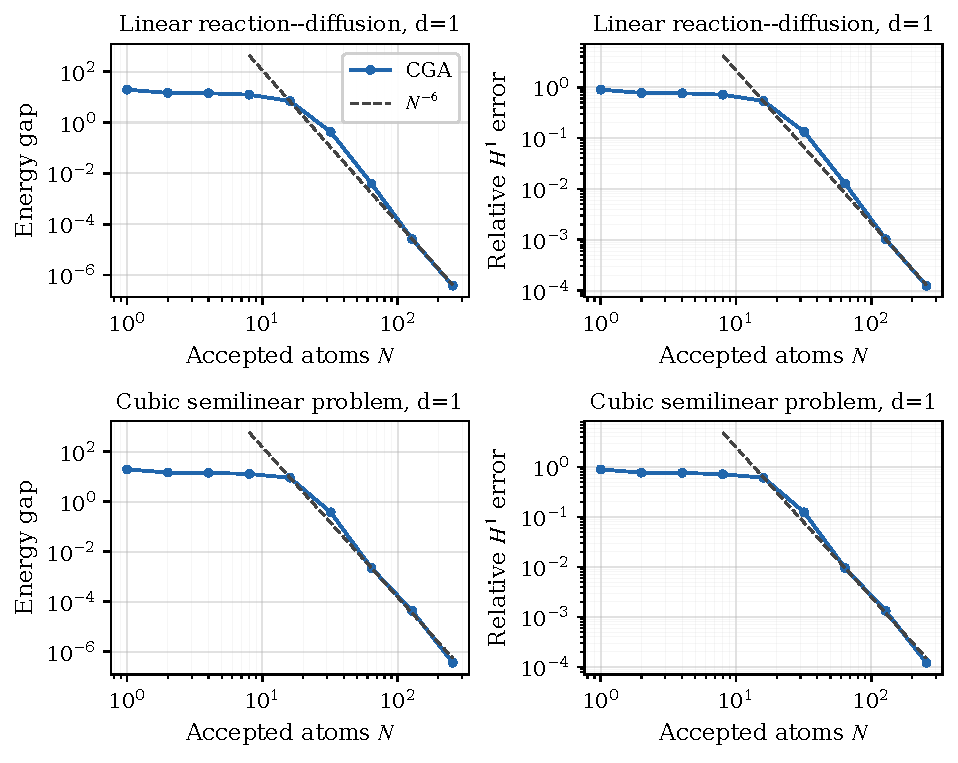
\includegraphics[width=0.96\textwidth]{cga_linear_cubic.pdf}
\caption{CGA values at retained powers of two for the linear and cubic problems. Each dashed segment
is the corresponding metric-specific conditional reference rate of
the displayed conditional exponent, restricted to the displayed index range.}
\label{fig:cga-linear-cubic}
\end{figure}

The two-dimensional sinh case is reported in the supplementary figures.  Its relative \(H^1\) error
decreases from \(4.074\times10^{-3}\) at \(N=256\) to \(1.990\times10^{-3}\) at \(N=512\), while the
local order decreases from 1.793 on \(128\to256\) to 1.034 on \(256\to512\). The final interval
therefore exhibits slower decay than the preceding interval.
\FloatBarrier

\subsection{Numerical results for the pure and regularized \texorpdfstring{\(p=4\)}{p=4} models}

\Cref{fig:cga-p4-representative} presents the one- and two-dimensional pure \(p=4\) cases using energy,
relative \(W^{1,4}\) error, and relative \(V\)-distance. The one-dimensional case reaches relative errors
\(1.579\times10^{-5}\) in \(W^{1,4}\) and \(1.680\times10^{-6}\) in the \(V\)-distance at its last
dyadic state \(N=128\). For the two-dimensional pure \(p=4\) problem, the interval \(128\to256\) has energy and \(V\)-orders 3.410 and
1.703.  On the final interval the \(V\)-distance continues to decrease, but the relative \(W^{1,4}\)
error increases from \(2.494\times10^{-3}\) to \(3.601\times10^{-3}\). Thus the terminal
Sobolev-error behavior is nonmonotone even though the \(V\)-distance decreases.

\begin{figure}[!htbp]
\centering
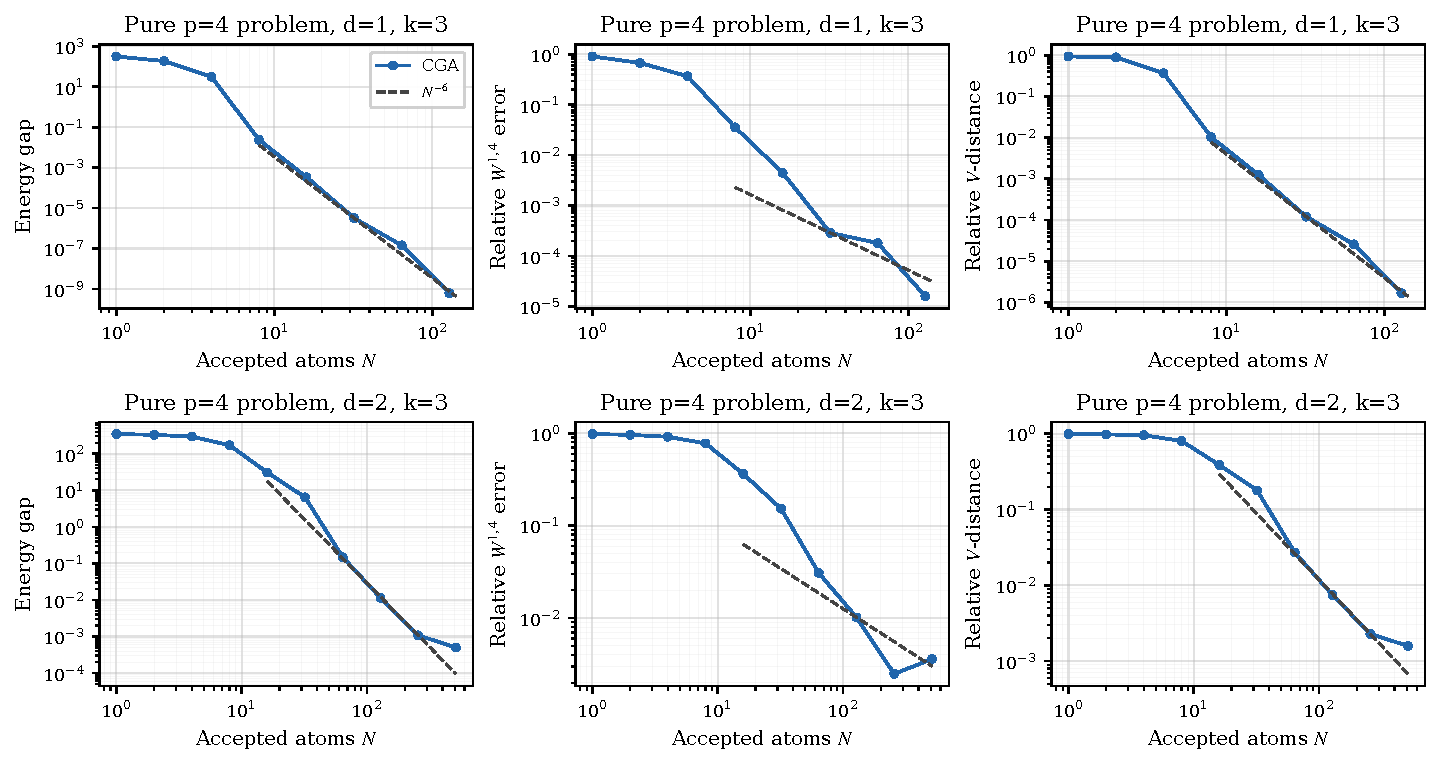
\includegraphics[width=0.98\textwidth]{cga_p4_representative.pdf}
\caption{CGA values at retained powers of two for the representative one- and two-dimensional pure \(p=4\) problems. The
three columns show energy gap, relative \(W^{1,4}\) error, and relative \(V\)-distance. Dashed segments
use the metric-specific conditional exponents stated above.}
\label{fig:cga-p4-representative}
\end{figure}

The dyadic values for the semilinear and $p=4$ cases are supplied in the supplementary numerical records. The regularized and reaction trajectories show the same separation between the natural-distance and Sobolev metrics as the representative pure cases.

\FloatBarrier

\subsection{Finite-trajectory checks for the quartic models}
\label{sec:finite-trajectory-numerics}
\label{sec:fractional-innovation-p4}

We evaluate the projection and quartic estimates of \Cref{sec:c5} on the
one-dimensional pure and regularized $p=4$, $k=3$ trajectories with
$u^*(x)=\cos(2\pi x)$ and $\varepsilon=0$ or $0.1$. The constants are
calibrated on the computed approximations at $N=8,\ldots,32$ and then held fixed on the
continuation to $N=64$. The calibration and continuation ranges are kept
separate, so the latter is only a finite-range check.

On the calibration range, the quartic identity and the projection-drop
identity agree with the computed values to floating-point accuracy under two
quadrature orders. The source and quartic comparison bounds cover the
computed energy errors in both models, although their terminal constants are
conservative. For the prescribed benchmark $\alpha=6$, the resulting
finite-range comparison powers are
\begin{align*}
 \widehat\delta_{8+j}&=O(j^{-6}),&
 d_{V,\bullet}(\widehat G_{8+j},u^*)&=O(j^{-3}),\\
 \|\widehat G_{8+j}-u^*\|_{W^{1,4}}&=O(j^{-3/2}),&
 1&\le j\le24.
\end{align*}
These are conditional envelopes on the calibrated range and do not assert an
asymptotic rate. The normalized-innovation condition remains satisfied for
27 of 32 continuation transitions in the pure model and 28 of 32 in the
regularized model; the exceptions prevent extending the same fixed-constant
bound to the whole continuation.

The detailed per-state source quantities, Hessian margins, quadrature checks,
and continuation records are supplied in the supplementary numerical files.


\section{Equal-DOF baseline comparisons}
\label{sec:results}

\subsection{Comparison setup and scope}

Five cases use a common evaluator: the one-dimensional linear problem, the one-dimensional cubic
problem, the two-dimensional sinh problem, the one-dimensional pure \(p=4\) problem, and the
two-dimensional pure \(p=4\) problem. The comparison variable is the number of independent global
coefficients: retained atoms for CGA, ridge features held fixed for RFM, and independent
finite-element coefficients after the constant mode is removed where required. Equal degrees of
freedom (DOF) do not imply equal runtime, memory, score evaluations, or nonlinear solver work, and
no cross-method timing conclusion is drawn from runs performed in different environments.
The supplementary numerical data at
\href{https://github.com/RonzolYu/cga4PDE}{\texttt{github.com/RonzolYu/cga4PDE}} give the prescribed realization count, the
available converged realizations, and the solver status for each width.

FEM uses continuous Lagrange elements on uniform one-dimensional meshes or structured triangular
two-dimensional meshes.  P1 and P3 provide low- and high-order mesh-based references in the main
figures. P2 results are retained in the supplementary material. P3 is the most accurate among the tested uniform-mesh FEM variants
at each largest common coefficient count reported below. The linear and cubic FEM curves are close
at high resolution, which is consistent with the common manufactured profile and an \(H^1\) error
dominated by the finite-element approximation.

For each case, the RFM uses a nested family of normalized \(\relu^3\) ridges and fits the outer
coefficients. Ten random-feature realizations are prescribed for each problem and width. Curves show the median and
interquartile range over solver-successful realizations at each width; the prescribed denominator and solver status
are listed in the supplementary numerical records. All ten realizations reach the displayed ranges for the linear,
cubic, sinh, and one-dimensional pure \(p=4\) problems. In the two-dimensional pure \(p=4\) problem,
seven of ten prescribed realizations succeed at \(N=128\) and four of ten at \(N=256\); consequently its
statistical curve ends at 256 and its terminal band uses those successful realizations. No distributional statement
is made at \(N=512\).

The CGA and RFM comparison curves join the computed powers of two listed in the numerical setup and the
terminal retained state needed to define the largest common comparison width, while FEM uses its own mesh degrees of
freedom. The figures contain no common-grid interpolants, theoretical reference lines, or
convergence-order-versus-DOF curves. The reported panel range ends at the terminal CGA width fixed
by the stopping rule, so that endpoint is determined by the stopping rule and the available method
states rather than by the plotted error values. Each method is shown only over the states it
actually reached. The equal-DOF tables use linear interpolation of log(error) against log(DOF)
between adjacent computed values when an exact coefficient count is unavailable; no extrapolation
is used.

The training, evaluation, and refinement quadratures are fixed as specified in the
supplementary protocol; all comparisons use the common DOF set
$8,16,32,64,128,256$, with $512$ used only when every method is bracketed by computed states.

\subsection{Evaluation and statistical samples}

The comparison errors use the fixed evaluation quadrature specified in the supplement, separately from
the quadrature used to construct the features and fit their coefficients. RFM medians and
quartiles are computed for each metric from successful coefficient solves with finite values
of that metric. All ten prescribed realizations contribute at the displayed C1--C4 widths. For C5,
seven of ten solves succeed at $N=128$ and four of ten at $N=256$; unsuccessful solves
remain in the prescribed denominator.

A separate supplementary evaluation contains 617 states satisfying its acceptance and
coefficient-count checks. Its signed energy/metric filter admits 611 of 617 states, its
\(H^1\)-dual residual filter admits 394 of 617, and its two-dimensional Bregman-integration
check admits 137 of 138. These counts refer to that separate collection; they do not define
the samples underlying the RFM curves or endpoint table in this section.


\subsection{Relative Sobolev errors}

For the linear, cubic, and sinh problems,
\Cref{fig:baseline-sobolev-1d,fig:baseline-sobolev-rest} report the relative \(H^1\) error. For the
two pure \(p=4\) problems, the corresponding panels report the relative
\(W^{1,4}\) error. These are Sobolev errors; the natural \(V\)-distance is reported separately below.

\begin{figure}[!htbp]
\centering
\subfloat[Linear, \(d=1\).]{%
\begin{minipage}[t]{0.49\textwidth}
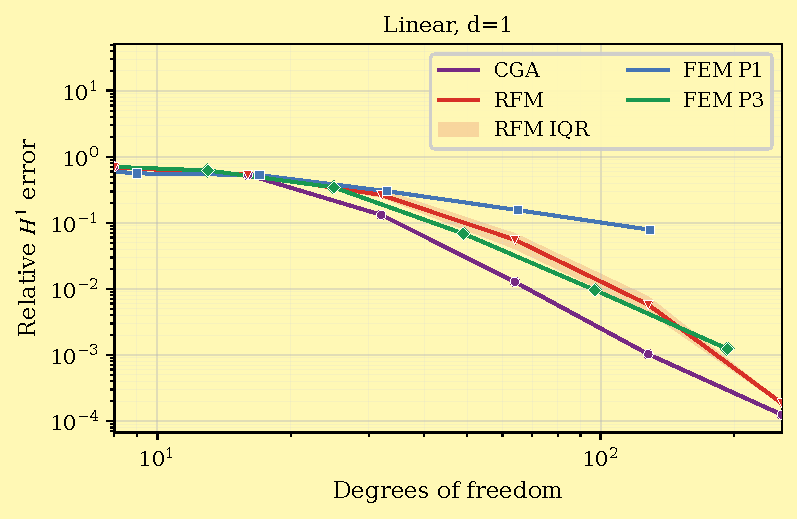
\includegraphics[width=\linewidth]{C1_relative_h1_error.pdf}
\end{minipage}}\hfill
\subfloat[Cubic, \(d=1\).]{%
\begin{minipage}[t]{0.49\textwidth}
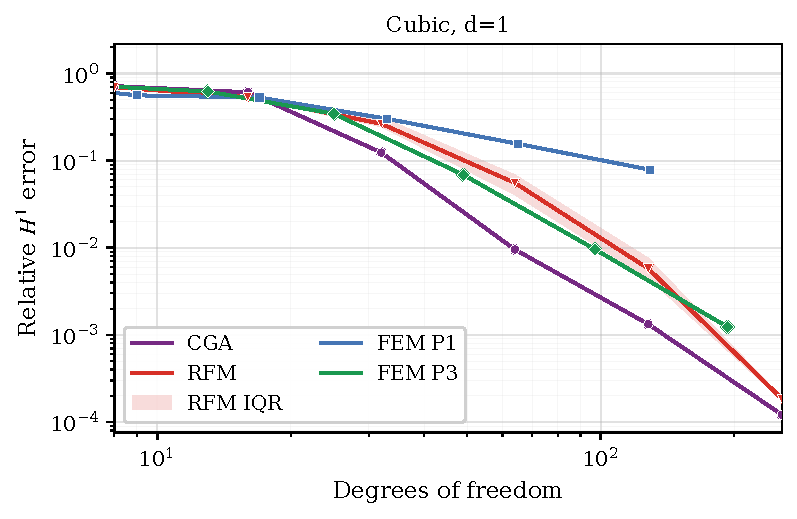
\includegraphics[width=\linewidth]{C2_relative_h1_error.pdf}
\end{minipage}}
\caption{Relative \(H^1\) error versus effective degrees of freedom for the one-dimensional
multifrequency problems. RFM curves show medians and interquartile bands over solver-successful realizations
from ten prespecified seeds. All markers are computed states.}
\label{fig:baseline-sobolev-1d}
\end{figure}

\begin{figure}[!htbp]
\centering
\subfloat[Sinh, \(d=2\): relative \(H^1\) error.]{%
\begin{minipage}[t]{0.32\textwidth}
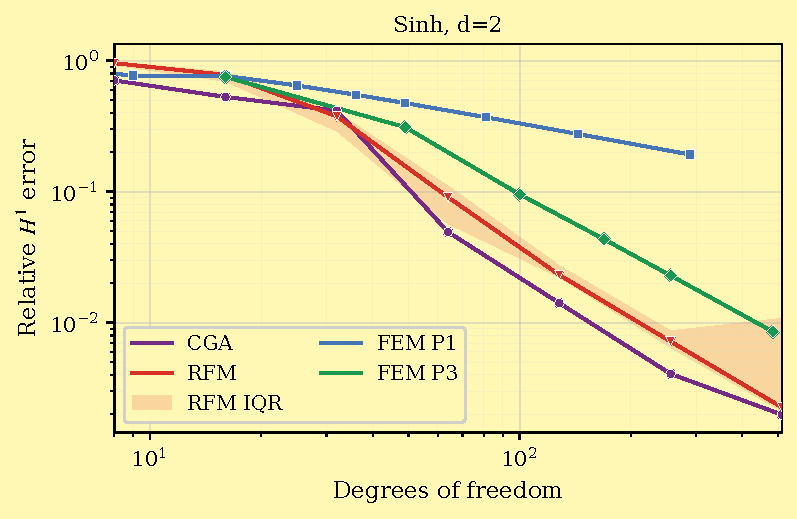
\includegraphics[width=\linewidth]{C3_relative_h1_error.pdf}
\end{minipage}}\hfill
\subfloat[Pure \(p=4\), \(d=1\): relative \(W^{1,4}\) error.]{%
\begin{minipage}[t]{0.32\textwidth}
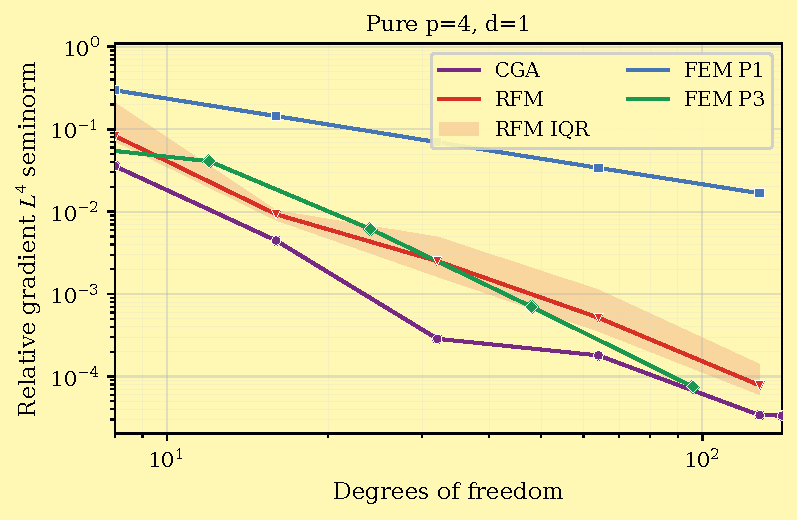
\includegraphics[width=\linewidth]{C4_relative_w1p_error.pdf}
\end{minipage}}\hfill
\subfloat[Pure \(p=4\), \(d=2\): relative \(W^{1,4}\) error.]{%
\begin{minipage}[t]{0.32\textwidth}
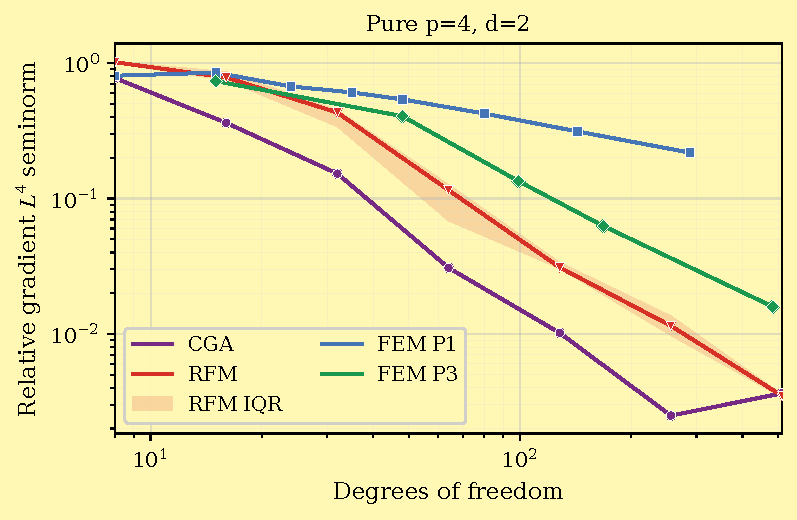
\includegraphics[width=\linewidth]{C5_relative_w1p_error.pdf}
\end{minipage}}
\caption{Relative Sobolev errors for the two-dimensional sinh problem and the pure \(p=4\) problems.
The two-dimensional pure \(p=4\) RFM band uses the seven solver-successful realizations at \(N=128\) and the
four solver-successful realizations at \(N=256\), with ten prescribed seeds at each width.}
\label{fig:baseline-sobolev-rest}
\end{figure}
\FloatBarrier

At the largest common endpoint supported by the configured RFM widths and bracketing FEM states,
CGA has the smallest relative Sobolev error in the linear, cubic, sinh, and one-dimensional pure
\(p=4\) problems; all ten prescribed RFM solves succeed in these four cases. The RFM-median/CGA ratios
are 1.49, 1.52, 1.77, and 5.76, and the P3/CGA ratios are 4.24, 4.35, 5.64, and 1.88. In the
two-dimensional pure \(p=4\) problem the successful-run RFM median and the P3 value are also above the
CGA value, by factors 5.01 and 16.12, respectively. The two-dimensional RFM statistics use seven of ten prescribed realizations at \(N=128\) and four of ten at \(N=256\) after solver-success filtering. These are endpoint comparisons
at equal coefficient count. The curves cross at smaller widths in some cases, so the data do not support
uniform dominance at every DOF.

\begin{table}[!htbp]
\centering\scriptsize
\caption{Relative $H^1$ error for C1--C3 and relative gradient $L^4$ seminorm for C4--C5 at the prescribed common coefficient counts. RFM statistics are median [Q1,Q3] over metric-valid realizations from ten prescribed seeds. Valid means a successful solve, a finite nonnegative metric, and an at-most-one-percent successive-quadrature difference for that metric; incomplete groups are conditional comparisons. Ratios larger than one favor CGA.}
\label{tab:baseline-terminal}
\resizebox{\linewidth}{!}{%
\begin{tabular}{@{}crrrrrr@{}}
\toprule
Problem & DOF & CGA & RFM median [Q1,Q3] & Valid & RFM/CGA & FEM P3/CGA \\ \midrule
Linear, d=1 & 256 & $1.247\!\times\!10^{-4}$ & $1.853\!\times\!10^{-4}$ [$1.779\!\times\!10^{-4}$, $1.913\!\times\!10^{-4}$] & 10/10 & 1.49 & 4.24 \\
Cubic, d=1 & 256 & $1.215\!\times\!10^{-4}$ & $1.853\!\times\!10^{-4}$ [$1.779\!\times\!10^{-4}$, $1.913\!\times\!10^{-4}$] & 10/10 & 1.52 & 4.35 \\
Sinh, d=2 & 256 & $4.074\!\times\!10^{-3}$ & $7.196\!\times\!10^{-3}$ [$6.472\!\times\!10^{-3}$, $8.663\!\times\!10^{-3}$] & 10/10 & 1.77 & 5.63 \\
Pure p=4, d=1 & 128 & $3.395\!\times\!10^{-5}$ & $7.818\!\times\!10^{-5}$ [$6.046\!\times\!10^{-5}$, $1.400\!\times\!10^{-4}$] & 10/10 & 2.30 & 0.88 \\
Pure p=4, d=2 & 256 & $2.493\!\times\!10^{-3}$ & $1.147\!\times\!10^{-2}$ [$9.730\!\times\!10^{-3}$, $1.360\!\times\!10^{-2}$] & 6/10 & 4.60 & 14.54 \\
\bottomrule
\end{tabular}}
\end{table}

\FloatBarrier

\subsection{Natural \texorpdfstring{\(V\)}{V}-distance for the \texorpdfstring{\(p\)}{p}-models}

\Cref{fig:baseline-v} repeats the two pure \(p=4\) comparisons with the relative \(V\)-distance defined in
\Cref{sec:numerics}.  Keeping this geometry separate from the \(W^{1,4}\) error is important because the
two quantities need not have the same terminal behavior.  The figure uses the same computed-state and
RFM uncertainty conventions as the Sobolev panels.

\begin{figure}[!htbp]
\centering
\subfloat[Pure \(p=4,d=1\).]{%
\begin{minipage}[t]{0.49\textwidth}
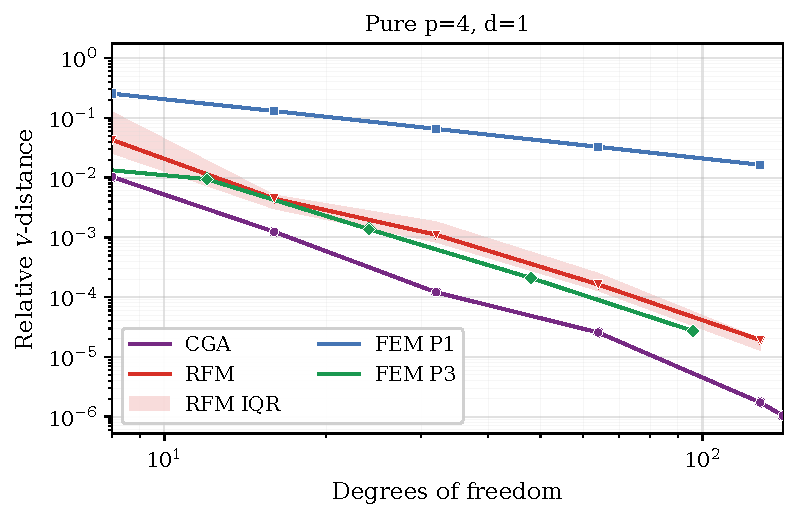
\includegraphics[width=\linewidth]{C4_v_distance.pdf}
\end{minipage}}\hfill
\subfloat[Pure \(p=4,d=2\).]{%
\begin{minipage}[t]{0.49\textwidth}
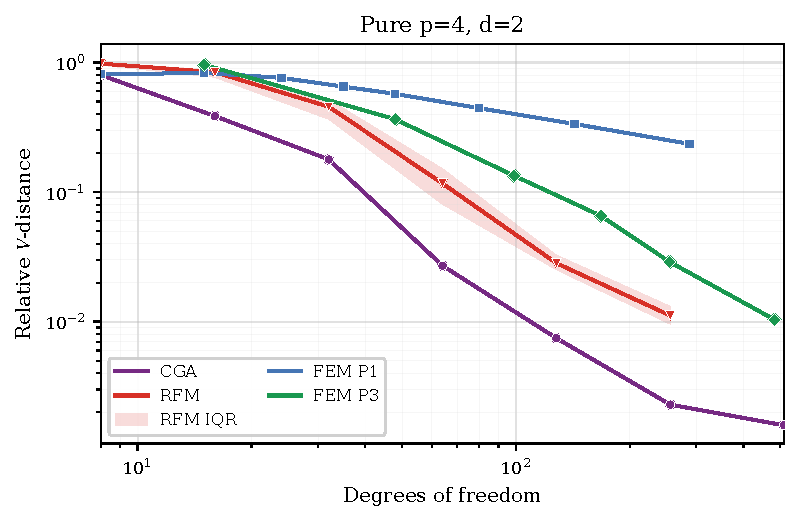
\includegraphics[width=\linewidth]{C5_v_distance.pdf}
\end{minipage}}
\caption{Relative \(V\)-distance versus effective degrees of freedom.  No theoretical reference line
or common-grid interpolation is drawn.}
\label{fig:baseline-v}
\end{figure}
\FloatBarrier

\subsection{Interpretation limits}

The equal-DOF results compare finite-pool CGA with the specified FEM and RFM methods.  They do
not establish a runtime ordering, do not compare CGA with every randomized or greedy dictionary method,
and do not turn endpoint ratios into asymptotic complexity estimates. The two-dimensional pure
\(p=4\) RFM summaries use
four of ten solver-successful realizations at the terminal width and are not a complete ten-seed
statistical comparison. Supplementary energy-gap comparisons are more sensitive to quadrature because they
subtract two separately integrated energies. The supplementary numerical data specify the prescribed and
converged realization counts, interpolation brackets, and computed coefficient counts.

\section{Discussion and conclusion}
\label{sec:discussion}

This work develops a unified variational framework for the analysis of finite-pool
Chebyshev greedy algorithms (CGA) for nonlinear PDEs. The atomic source condition and
directional smoothness yield an $O(m^{-1})$ energy bound for the ideal
continuous-dictionary CGA. For the practical finite-pool algorithm, the analysis further
separates the effects of continuous-dictionary coverage, score-evaluation error, radial
stationarity, and inexact coefficient optimization, and identifies relative accuracy
conditions under which the same energy order is retained. This provides a quantitative
description of how finite-pool approximation, numerical score evaluation, and inexact
active-space solves influence the greedy descent mechanism.

For the standard pure, regularized, and reaction $p$-energies with $p\geq2$, we further
establish quantitative relations among the energy gap, the natural $V$-distance, and the
Sobolev error. In particular, an energy exponent $\alpha$ leads to the corresponding
natural-distance and $W^{1,p}$-error exponents $\alpha/2$ and $\alpha/p$, respectively.
This allows energy estimates for the greedy algorithm to be translated directly into error
measures adapted to the nonlinear geometry of the underlying PDEs.

Building on this structure, two refined analytical mechanisms are developed. The local
Hessian-transfer analysis connects the nonlinear problem with greedy approximation in a
frozen Hilbert metric, while the finite-trajectory analysis works directly with the nested
spaces generated by the computation and produces explicit projection bounds through either
an approximate source representation or normalized innovations. For the quartic energy, an
exact energy decomposition further connects these projection estimates with nonlinear
energy errors. Consequently, even on computational ranges where a uniform asymptotic
theory is not yet available, the analysis provides quantitative and directly testable
explanations of the observed algorithmic trajectories.

The one-dimensional pure and regularized $p=4$ experiments support this
finite-trajectory framework. On the calibration range $N=8$--$32$, both the
source-based and fractional-innovation bounds enclose the computed errors.
For the prescribed benchmark $\alpha=6$, the conditional comparison powers
on this range are $6$, $3$, and $3/2$ for the energy, natural distance, and
$W^{1,4}$ error, respectively. The projection and quartic identities remain
accurate under two quadrature rules on the continuation to $N=64$.
The normalized-innovation sufficient condition holds for 27 of 32 continuation
transitions in the pure model and 28 of 32 in the regularized model.
Numerical coverage by a conservative expression on the continuation does not
establish the same theorem guarantee throughout that range.

The equal-coefficient comparisons use refitted CGA prefixes and fully
archived FEM and RFM states with the same metric-specific quadrature policy.
Their computed CGA and RFM endpoints, together with interpolated FEM reference
values where indicated, describe the approximation errors for the specified problems and valid samples. They do not establish uniform superiority over
all widths, excluded realizations, or computational-work budgets. The
componentwise gradient seminorm, full Sobolev norm, and natural distance are
reported as distinct metrics rather than interchangeable relative errors.

Overall, the theoretical and numerical results show that finite-pool CGA admits a coherent
variational analysis while providing effective low-dimensional adaptive approximations for
nonlinear PDEs with $p$-structure. The present framework also identifies concrete and
testable conditions for further developments, including continuous-dictionary coverage,
entropy bounds for the restarted dictionary, and invariance of the Hessian neighborhood.
Establishing these conditions uniformly, together with reliable numerical enclosures and
comparisons under a common computational-work measure, would provide a natural route from
the present finite-range theory toward a more complete asymptotic convergence and
complexity theory.

\section{Code and data availability}
\label{sec:code-data}

Code and data are publicly available at \url{https://github.com/RonzolYu/cga4PDE}.
The comparisons use the \texttt{review\_replay\_20261001} batch and
\nolinkurl{code/config/review_replay.json}. Each comparison state has a
coefficient model/hash, evaluation rule, and metric-specific audit. Historical
records remain separate. The README and S3--S4 specify sample definitions and
distinguish artifact rebuilding, saved-model reevaluation, and fresh coefficient
fits.


% The source-class proof is supplied in
% supplement/S4_background_details/A_source_proof_full.tex to keep the main
% manuscript within the SISC length policy.

\bibliographystyle{siamplain}
% DOI metadata remains in the BibTeX source; suppressing printed URLs keeps the
% reference list within the SISC page limit without changing citation identity.
\begingroup
\renewcommand{\url}[1]{}
\bibliography{References/references}
\endgroup

\end{document}
